\documentclass[10pt]{article}
% \usepackage[margin=1in]{geometry}
% \newcommand\hmmax{0}
% \newcommand\bmmax{0}

% % % Fonts% %
\usepackage[T1]{fontenc}
   % \usepackage{textcomp}
   % \usepackage{newtxtext}
   % \renewcommand\rmdefault{Pym} %\usepackage{mathptmx} %\usepackage{times}
\usepackage[complete, subscriptcorrection, slantedGreek, mtpfrak, mtpbb, mtpcal]{mtpro2}
   \usepackage{bm}% Access to bold math symbols
   % \usepackage[onlytext]{MinionPro}
   \usepackage[no-math]{fontspec}
   \defaultfontfeatures{Ligatures=TeX,Numbers={Proportional}}
   \newfontfeature{Microtype}{protrusion=default;expansion=default;}
   \setmainfont[Ligatures=TeX]{Minion 3}
   \setsansfont[Microtype,Scale=MatchLowercase,Ligatures=TeX,BoldFont={* Semibold}]{Myriad Pro}
   \setmonofont[Scale=0.8]{Atlas Typewriter}
   % \usepackage{selnolig}% For suppressing certain typographic ligatures automatically
   \usepackage{microtype}
% % % % % % %
\usepackage{amsthm}         % (in part) For the defined environments
\usepackage{mathtools}      % Improves  on amsmaths/mtpro2
\usepackage{amsthm}         % (in part) For the defined environments
\usepackage{mathtools}      % Improves on amsmaths/mtpro2

% % % The bibliography % % %
\usepackage[backend=biber,
  style=authoryear-comp,
  bibstyle=authoryear,
  citestyle=authoryear-comp,
  uniquename=false,%allinit,
  % giveninits=true,
  backref=false,
  hyperref=true,
  url=false,
  isbn=false,
  ]{biblatex}
\DeclareFieldFormat{postnote}{#1}
\DeclareFieldFormat{multipostnote}{#1}
% \setlength\bibitemsep{1.5\itemsep}
\newcommand{\noopsort}[1]{}
\addbibresource{Thesis.bib}

% % % % % % % % % % % % % % %

\usepackage[inline]{enumitem}
\setlist[itemize]{noitemsep}
\setlist[description]{style=unboxed,leftmargin=\parindent,labelindent=\parindent,font=\normalfont\space}
\setlist[enumerate]{noitemsep}

% % % Misc packages % % %
\usepackage{setspace}
% \usepackage{refcheck} % Can be used for checking references
% \usepackage{lineno}   % For line numbers
% \usepackage{hyphenat} % For \hyp{} hyphenation command, and general hyphenation stuff
\usepackage{subcaption}
% % % % % % % % % % % % %

% % % Red Math % % %
\usepackage[usenames, dvipsnames]{xcolor}
% \usepackage{everysel}
% \EverySelectfont{\color{black}}
% \everymath{\color{red}}
% \everydisplay{\color{black}}
% % % % % % % % % %

\usepackage{pifont}
\newcommand{\hand}{\ding{43}}
\usepackage{array}


\usepackage{multirow}
\usepackage{adjustbox}

\usepackage{titlesec}

\makeatletter
\newcommand{\clabel}[2]{%
   \protected@write \@auxout {}{\string \newlabel {#1}{{#2}{\thepage}{#2}{#1}{}} }%
   \hypertarget{#1}{#2}
}
\makeatother

\usepackage{multicol}

\setcounter{secnumdepth}{4}
\setcounter{tocdepth}{4}

\usepackage{tikz}
\usetikzlibrary{arrows,positioning}

\usepackage{tabularx}

\usepackage{bussalt}

\usepackage{Oblique} % Custom package for oblique commands
\usepackage{CustomTheorems}



\usepackage[hidelinks,breaklinks]{hyperref}

\title{Oblique Reasoning}
\author{Ben Sparkes}
% \date{ }


\begin{document}

\section*{Notes}



\begin{itemize}
\item Scenarios for informal descriptions, diagrams for use of the formal tools.
\item Settling involves answering and guessing
  \begin{itemize}
  \item Further, settling doesn't necessarily involve using information; the extreme case of guessing as rolling die, etc.
  \end{itemize}
\end{itemize}

\begin{itemize}
\item Idea that something like a profile is needed, as there's no way to choose between individual options.
\item Right, the idea here is that there's nothing like choice involved, in some sense.
\item More broadly, the idea is that there are cases in which something happens in the world and I can update based on this, it's a probability distribution, right.
  And, if one is sensitive to these kinds of issues then \dots it still seems as though there's not much to be done by way of probability here.
  For, one can't do much other than condition.
\end{itemize}

\newpage

\begin{enumerate}
\item Scenarios
  \begin{enumerate}
  \item Shops, as this is the simplest
  \item And another slightly more complex scenario, to show the potential complexity of the reasoning and the use of some detailed means that build.
  \end{enumerate}
\item The interest here is in reasoning leading to action that you pursue despite being unable to evaluate the desirability of relevant action.
\item This contrasts with cases in which you can remember the end but not the means.
  \begin{itemize}
  \item For example, going to the shops and forgetting where the milk is.
  \end{itemize}
\item So, the contrast is to standard means-end reasoning.
\end{enumerate}



The simple view that I'm arguing against is that one acts on the basis of their evaluation of ends.
So, if one acts, then there is an end to that action which they evaluate.
One acts on the basis of practical reaosning if there is some evaluate end that the action is a means to.
(Where, the end itself is trivially a means to the end.)
This is often a sound inference to draw.
I'm picking up items in the supermarket, and it's reasonable to think that I have something that I'm going to do with these.
Right, the basic idea is that if some practical reasoning has taken place, then I have identified some end, and the actions are being performed as a means to that end, and so there's an evaluative judgement in favour of the end.

\begin{quote}
  If an action is being perfomed on the basis of reasoning about what to do, then some evaluative attitude has been established in favour of this action over other actions, and this evaluation depends on an evaluation of an end to which the action is a means.
\end{quote}
Here, the important thing is that this is all within the same piece of reasoning.
The basic argument would be that you're performing the action as a means to some end, and it seems quite strange that the evaluation of the means could be independent.
The action is a means, if its significance was not due to the evaluation of an end, then this action would be an end in itself.
This, then, seems like a quite general truth.
The dependency really is key, as if not, then the evaluation for the means holds regardless of the end, and so instead the means should be considered as an independent end.
Instead, the agent has a sequence of desirable actions.
For example, listening to music and going for a run.
Going for a run could be a means to listen to music, if I would otherwise do something else.
However, if I'm going to listen to music and it's also the case that I can do this while running.
Means-end structure does not follow from piecing together a sequence of desirable actions.

Of course, means-end is slightly ambiguous, but it's about some structured reasoning rather than possible dependencies, etc.

So, from this dependency relation, one may think that when acting on the means to an end, an agent must be able to reason about the relevant end.
For, else the agent cannot determine an important part of the desirability of the means.

Used to thinking about idealised agents, but even if we relax assumptions about the ability to canvas all reasons for action (whether these be desires or something else), acting on a means as a means without being able to determine the reasons for the end, would be puzzling.

Have cases where we forget the end but act on the means.
So, either this link breaks down, and it's possible to act on means independent of the end, reasoning about the desirability of the end need not be direct, or there is some substitute end that can be reasoned about.

The first option will not be pursued.
Maybe there is a good argument for this, but I do not see a way to understand means-end reasoning without this dependency requirement.
And, in the relevant cases, it really does seem as though this dependency is preserved.

The third option also seems implausible.
Sometimes there may be a substitute, but this is usually when a certain way of representing fails.
Sometimes one goes via indirect reference, for example.
Want to see some specific movie, and then move to a kind of definite description.
So long as the description retains enough of the characterisitics, then you're probably fine.
In the cases of interest, the only reasonable substitute is the end to which the means is a means.
Yet this doesn't seem to help, for there's no way to get enough information to figure out the relevant end.
However, two cases to distinguish, as `mode of presentation' may be though to make a difference.
Here, however, I'm assuming it does not, and if it does then this only strenghens the problem.
\begin{itemize}
\item The idea about a substitute end can also be rephrased in terms of the evaulation of the means being all that's required, so you forget the end, but the relevant evaluation of the means is preserved, and this does enough for you to pursue the means, as nothing in the background has changed, etc.
\item This seems strange, though, as the dependency between means and end suggests that this can't be all that's going on.
\item So, one could think that evaluation attaches to representation and that it's then a matter of deciding between these.
\item I mean, in part this seems natural as it `shouldn't' be the case that there's a way to increase the desirability of means due to some decision, but this seems problematic to the degree that decisions do have this property.
\end{itemize}

\begin{itemize}
\item Another way of stressing the core idea above is that the relevant dependency is key to understanding the reasoning, and it doesn't make sense to think that the same action which serves as the means would have been chosen were it not for the end that led to the evaluation.
\item So, a key part of the reasoning is that there \emph{is} this dependency.
\item And, this dependency means that you're not able to figure out the present desirability, etc.
\item Needs to be some care here, as, for example, \citeauthor{Bratman:1987aa} argues that in the case of intention, where this kind of means-end reasoning is clear, that there's no change in the desirability of the options, and instead there's some kind of filter of admissibility.
\item Idea of a filter is neat, and as this is independent of desire (or whatever) it's not too hard to imagine that this could be preserved.
  \begin{itemize}
  \item However, problem is that without the end, there doesn't seem to be a sufficient grasp on admissible options.
  \item That is, the agent may do things that would otherwise be inadmissible in pursuit of the oblique pursuit of the end.
  \item Right, the basic idea with the filter is that it rules out options, and so the idea that this persists can't be right, though the functional idea of a filter could remain, in the sense that there's some constraints and some reverse inference going on, but whatever the filter \emph{was} can't persist.
  \item For exmaple, going to the shops, filter should be that you go straight to the right section, but this doesn't happen without the end.
  \end{itemize}
\item So, overall idea here is that filters seem interesting because they capture some of this dependency structure, but they rely too much on a `controlling' representation.
\end{itemize}


So, second option.
Rest of the paper is exploring this.
\begin{itemize}
\item Descriptive: what's going on, and how does this affect understanding of practical reasoning?
\item Normative: what does rationality say about such cases?
  \begin{itemize}
  \item Here, one might expect there to be a whole buch of stuff that comes into play with respect to lack of information.
  \item That is, one starts to wonder about the quality of the information they have, rather than the mere presence of information.
  \item In some respects, this may be the easier argument to make.
  \item And not only quality; the way in which one is reasoning seems important too.
  \end{itemize}
\end{itemize}

On the descriptive side, the question is about using reasons that one doesn't have direct access to.
Noramtive questions are going to most likely be postponed, but to note is that this kind of reasoning doesn't seem irrational, though this may be due to the fact that these are practical issues.
That is, question as to whether this can be transferred over to beliefs, etc.

\begin{itemize}
\item On the descriptive side, the diagrams basically explore the relation between what the agent's reasons determine and what they're able to represent.
\item In some respects this is kind of impoverished, but this is where the focus is, you can create a heirarchy of reasons, for sure, but fix something relevant.
\item Also referntial as this makes things a lot more straightforward, likewise for the satisfactory/unsatisfactory binary distinction.
\end{itemize}


\begin{itemize}
\item Parts of the descriptive argumnet:
  \begin{enumerate}
  \item Have two variables, at least, and the less information you have connecting these, the easier it is for them to come apart.
  \end{enumerate}
\end{itemize}


\begin{itemize}
\item Strong principle: the ability to evaluate means requires the ability to evaluate the end to which it is a means.
  \begin{itemize}
  \item This I do not think can be the case.
  \end{itemize}
\item Weaker: the ability to evaluate means requires the ability to have had evaluated the end to which it is a means.
  \begin{itemize}
  \item This I don't have an argument against.
  \end{itemize}
\end{itemize}


However, it then seems as though if one is unable to evaluate the end to the means they are considering, then they cannot appropriately evaluate the means, and hence the action performed must be its own end.

\section{Argument outline}
\label{sec:argument-outline}

\begin{enumerate}
\item dependency
\item means settle
  \begin{enumerate}
  \item settling is a formal notion, so there's no avoiding this, means still provide information, etc.
  \item Note, settling is something the agent does, it doesn't necessarily correspond with what the agent ought to do.
  \end{enumerate}
\item no access of end
\item settle via something else; something other than primary value
  \begin{enumerate}
  \item value is a formal notion here, so this idea of primary value is kind of important, as it distinguishes something of importance about means
  \item have a problem if settling only happens in accordance with primary value
    \begin{enumerate}
    \item this should have some precedence, but it's not clear it does, for it's usually the case that one simply needs to argue that the alternative has greater value.
      Should look at Smith, Bratman, and maybe others.
    \end{enumerate}
  \item This doesn't generalise to what the agent ought to do, as the focus here is on the agent's reasoning.
  \end{enumerate}
\end{enumerate}


\begin{itemize}
\item Natural thing to say here is that there's some kind of derived value that aims to keep track of primary value.
\item This is really the core idea, and it's a familiar idea, especially in the case of intentions.
\item But no intentions here, at least not in any robust sense.
\end{itemize}





\newpage

Two tools:
\begin{enumerate*}
\item attunement, and
\item compliance
\end{enumerate*}

Attunement: develop one's attitudes to accord with some standard.
Compliance: ensure that one's attitudes conform to structural constraints.

Are these the right concepts?
Think of Frankfurt.
Higher-order attitudes.
Here, it looks as though it's compliance, lower-order attitudes are constrained by higher-order attitudes.
It also kind of looks like attunement, as these set some standard, in a sense, but this is harder to see, as everything is more-or-less internal.
So, maybe the qualifier should be that the standard is independent of what's available to you in your reasoning.
This gives the possibility of a hybrid position, where higher-order attitudes aren't known, but it's not obvious that Frankfurt requires this.


\newpage
\maketitle

\section{Introduction}
\label{sec:introduction}

Four kilometres to go, the second left after the traffic lights, and a right shortly after.
Preparing the meal had been going well until \dots until \dots, well \emph{some} ingredient is missing.
The name of the ingredient was left on the fridge, but the ingredient is in the supermarket and you're sure that you'll recognise it when you see it, and you're confident you will.

Obtaining the missing ingredient is a means to cooking the meal which is in turn in service of some further end.
Isolated, obtaining the ingredient functions as an end and the supermarket is a means to that end.
Before you set out to the store you had a clear grasp on this end; you checked each item from the list until you came to what you have set out to obtain, and the missing item was so clear that you didn't bother to take a note.
Nearing the supermarket, you realise this may have been a mistake.
You could turn back, but you have a partial grasp on the end you are pursuing; going to the supermarket is a means to obtaining that ingredient, that ingredient is required to for this unspecified meal, and it was sufficiently familiar that you skipped making a note.
Achieving the end requires that you recall what the missing ingredient is, but it does not require that you're able to do so while cycling, nor does it require that you do so by looking at your fridge.
So long as you're able to find what you're looking for, it'll all be fine.
Later you return with the ingredient and prepare the meal.

Abstractly, an agent had some end, formed means to this end, and the relevance of those means persisted despite the agent losing track of the end.
The details are mundane.
Consider stumbling with 'ums\dots' and 'ahs\dots' as you try to recall what you wanted to say while recalling the initial fragment of your utterance or the pause as you walk into a room and the next step eludes you.
The utterance fragment and entry to the room were means to some end, and the information that those means provide often allow you to recover the end.
The way in which ends can be recovered be a black box throughout this paper.
Our interest in these scenarios is how and why certain means persist without an agent being in a position to evaluate the relevant end.
For, intuitively, when engaging in means-end reasoning, an agent's valuation of a means primarily depends on their valuation of some end.
So, if an agent loses track of the end, it seems they cannot track the value of means to that end.
Is continuing to purse the means rational?
If so, what descriptive and normative resources are required to analyse such scenarios, do these resources apply to other scenarios, and if so do they offer novel insights?

\begin{itemize}
\item Puzzle
\item Perspective
\item Reduction
\end{itemize}

The goal is straightforward.
To state what the puzzle is, to give a perspective on the puzzle, and to show the relation the puzzle bears to other topics in the philosophy of action given this perspective.

The perspective offered will draw on decision theory, but decision theory is not essential to what I have to say.
Decision theory offers a toolkit,

Much like an amateur artist with poster paints and cardboard, you may not like what is produced, nor how it is produced.
However, if the artist tries their best, then with your understanding of the medium you'll likely be able to figure out what they're getting at, and perhaps well enough to recreate with your own tools.

\newpage

\section{Basics}
\label{sec:basics}


Practical reasoning is settling the issue of what to do, and issues are settled by information.
So, practical reasoning amounts to the processing of information.
To put these sweeping statements to work, define information to be the elimination of situations, and identify actions with the situations which would result from their performance.
Practical reasoning then narrows down some range of situations to some action, or collection of actions to be performed.
Situations are represented and evaluated, and the evaluation of a situation is typically tied to its representation.
Two principal components of evaluation are whether a situation is possible, and whether a situation is worthwhile.
These components constitute information, as they determine whether a possibility is to be eliminated or not.

This is the model of practical reasoning at work in this paper.
It can be seen as a loosening of the folk-theoretic model which makes use of the propositional attitudes of belief and desires.
Beliefs provide information about what is possible, desires about what is worthwhile, and propositions may represent, or be represented.
Still, to talk of beliefs, desires, and propositions may suggest substantial commitments about the underlying metaphysics or everyday conception of practical reasoning.
Here we are interested in pure theory; theory which has useful and widely applied instantiations, but it is only the formal features of this core that matter here.
Likewise, information about what is possible may be captured by probabilities and what is worthwhile by utility, as in decision theory.

One may colloquially say that they used the information provided by their evaluation of how they represented the situations on the menu to eliminate those situations in which they ordered a meal other than the one they chose, but forget such colloquialisms.
Situations, representations, evaluations, and information are tools the we use to reason about scenarios and our use of these tools will is implicitly defined by the functional role we assign to them.
The focus of this paper is information; what is used to settle the issue of what to do, or alternatively, what is used eliminate situations?
The puzzle is about how means to an end can provide information without an agent being in a position to process information about the end.

In the opening scenario, the agent had the end of preparing a meal; some reasoning led them to evaluate preparing a meal as both possible and worthwhile.
Noticing that they lacked an ingredient, they saw obtaining that ingredient as possible and worthwhile.
Obtaining the ingredient may not have been necessary, for perhaps a substitute ingredient could have been used.
Still, if there was a substitute this either was not possible, or was not as worthwhile as obtaining the missing ingredient.
Hence, obtaining the ingredient became a means by which they would prepare the meal.
Again, the reasoned that going to the supermarket would be possible and worthwhile and so elaborated on their means to preparing the meal.
To keep things simple, we redescribe obtaining the ingredient as an end to which going to the supermarket is a means by treating the preparation of the meal as a background constraint on the agent's reasoning.
This allows us to focus on the agent's reasoning which is conducive to that constraint.
Preparing the meal was likely in the service of some prior end, and so long as we assume such prior ends remain in force we need not complicate matters with a complex hierarchy of means, likewise we omit additional reasoning about getting to the shops.\nolinebreak
\footnote{Treating the preparation of the meal as a background constraint is simply a convenience.
We would keep the preparation of the meal along with other situations in the foreground if we were to consider adjacent scenarios in which the agent may deviate from preparing the meal.}
The agent, then, has the end of obtaining some specific ingredient, and a means to that end.

The agent settled the issue of what to do in favour of going to the supermarket, and when there they can settle further issues by appeal to the information they used when they settled the issue of what to do in favour of obtaining the ingredient.
In a sense the issue of what to do is never settled, but only in the sense that one cannot settle on a largest natural number.
The problem arises when the agent lacks information they once had.
Forgetting the ingredient, the agent can no longer rule out situations in which they leave the supermarket without the ingredient they require, though they remain able to rule out situations in which the leave the supermarket without any ingredient.

The puzzle is why going to the supermarket still settles the issue of what to do.
Going to the supermarket is a means to the end of obtaining some ingredient, and is worthwhile primarily because obtaining the ingredient is worthwhile.
However, that that the agent requires \emph{some} ingredient doesn't make the supermarket more worthwhile than any of the other shops which sell ingredients, neighbours, or using a substitute.
For sure, at one point information was used to rule out situations such as these, but without that information the supermarket may appear less worthwhile than some other alternative.
{\color{red} More here, additional problem is that you can't really evaluate these options, as you can't represent the end.
  Though, part of the point here is that this is with the substitute end.}

{\color{green} Generalising a little, the puzzle here is complementary to questions raised by the idea of transformative experiences.
  There, you have a representation without being able to assign a value to it, while here you have some value without being able to represent it.
  Specifically, however, the puzzle relies on the value having been used in practical reasoning.
Perhaps unrecognised value is puzzling in general --- I am inclined to think so --- but this is a little more delicate, as there's something like complete ignorance here.}




A form of bootstrapping is nearby.\nolinebreak
\footnote{Footnote about the bootstrapping problem as it applies to intention, here the situation is somewhat similar, but in terms of either continuing to perform the action, or in terms of further deliberation.}
For, if the agent arrives at the supermarket, then the information the agent uses may settle what to do in favour of actions involving the supermarket.
However, that an action can influence an agent's evaluation of further actions is familiar.
Buridan's Ass need only take one step toward a bale in order to resolve it's parallel evaluations of the two equidistant and otherwise-seemingly-identical bales of hay.
Hence, whether further actions can be `bootstrapped' in a problematic way is derivative of whether the agent acts rationally by continuing to the supermarket.

In a different and more familiar sense, the agent may `bootstrap' going to the supermarket by using their prior adoption of the act as a means to some end to support going to the supermarket.
Analogous to bootstrapping in the case of intention, taking prior reasoning as a source of information may allow an agent to generate further `information' that would otherwise be unavailable.
For example, if an agent holds that the adoption of a means provides information that the end to the means is possible and more worthwhile than any other end, then the agent can discount any other end from settling what to do.
To see how this can be problematic, consider the following principle:\nolinebreak
\footnote{I take this principle to be fairly uncontroversial \dots
  \begin{quote}
    the value of the means derives from the value of the ends \dots
    If there are reasons to take the means, they must be none other than the reasons to pursue the ends, or at least they must derive from them.\nolinebreak
  \mbox{ }\hfill(\cite[2]{Raz:2005aa})
\end{quote}

\begin{quote}
  Consider cases of means-end rationality, that is, cases in which I form a desire to perform the means to an end because I have a background desire for that end and a belief that the means is a means to that end.\nolinebreak
  \mbox{ }\hfill(\cite[84]{Smith:2004aa})
\end{quote}

\begin{quote}
  Most objectives and activities derive their value from the means-ends relationships which connect them with objectives or activities that are valued in themselves.
  By a process of anticipation, the value inhering in the desired end is transferred to the means.\nolinebreak
  \mbox{ }\hfill(\cite[61]{Simon:1997aa})
\end{quote}

\begin{quote}
  Desire–Belief Theory of Reasoning: Desire that M is created as the conclusion of reasoning if and only if the reasoning combines desire that E with belief that M would raise E’s probability.
  It is eliminated as the conclusion of reasoning if and only if the reasoning eliminates such a combination.\nolinebreak
  \mbox{ }\hfill(\cite[2]{Sinhababu:2017aa})
\end{quote}

\begin{quote}
  The instrumental value of a means is not to be counted as additional to the intrinsic value of the end.
  (Otherwise, we would be obliged to pursue our ends as circuitously as possible, so as to accumulate the most instrumental value along the way.)
  Since the value of a means is not additional to that of the end, turning a misfortune into a means of learning a lesson doesn’t produce any more value than that inherent in the lesson itself, a value not necessarily greater than that of any alternative lesson one might have learned.\nolinebreak
  \mbox{ }\hfill(\cite[65]{Velleman:2000ab})
\end{quote}

\begin{quote}
  The ``will'' to attain an end is being transmitted to (use of) the means deemed necessary for its attainment.
  This principle of ``transmission of intention from ends to means'' is basically identical, it seems, with a principle which Kant thought analytically (logically) true and which he expressed in the following words:
  ``Who wills the end, wills (so far as reason has decisive influence on his actions) also the means which are indispensably necessary and in his power.''\nolinebreak
  \mbox{ }\hfill(\cite[40]{Von-Wright:1972aa})
\end{quote}
}
\begin{principle}\label{princip:dependency}
  When engaging in means-end reasoning, an agent's evaluation of a means primarily depends on their evaluation of the end to that means.
\end{principle}
The information used by an agent in settling a means derives from the information used in settling the end of that means.
So, to use the adoption of the means as information to settle what to do in favour of an end reduces to taking the information about the end as sufficient to settle what to do independent of any other option.\nolinebreak
\footnote{
  Roughly, at least.
  \begin{center}
    [Caveats]
  \end{center}
}

Given \citeauthor{Bratman:1987aa}'s early account of intentions (\citeyear{Bratman:1987aa}) where adopting an intention `filter's out' options incompatible with the intended option, then the above account of bootstrapping coincides with that as described by \citeauthor{Bratman:1987aa}, if we assume that agent forms an intention to perform the means to the end.

This early account of intention differs from later account in which intentions do provide information.

This would avoid the kind of bootstrapping under consideration, 



As things stand, however, we make no assumption about the role, if any, for intentions of any kind in our understanding of this puzzle.


The end is the boot, the means the strap, and the `information' generated is the irrelevance of other ways in which what to do may be settled.
Alternatively, no `information' is generated an the agent violates a principle governing the scope of their reasoning:
\begin{principle}\label{princip:global}
  Whether something settles the issue of what to do depends on evaluation of alternatives.
  (Something about settling being comparative.)
\end{principle}

Bootstrapping is problematic enough, and then you can't even represent which boot you're putting on!
{\color{red} Aside, the discussion applies to when other parts of evaluation fail.
Representation is something of a special case, it's not more general, though.}

Putting principles~\ref{princip:dependency} and~\ref{princip:global} together, whether some means settles what to do depends on how the end to the means compares to the agent's evaluation of alternatives.
Therefore, if an agent isn't able to evaluate the end to some means, then the agent cannot settle what to do in favour of the means.
And, it seems, if an agent cannot represent the end to their means, then they cannot evaluate that end without either generating illicit information or failing to engage in practical reasoning.
From this one may slip to the conclusion that an agent can only engage in practical reasoning with what they can represent, and that if an agent cannot represent the end to their means they cannot appropriately reason about their means \emph{as means to some end}.


\begin{principle}\label{princip:seperation}
  Whether something is worthwhile or possible is not necessarily a function of its representation.
\end{principle}
In other terms, a theory of practical reasoning in which it is possible to separate whether or not something is worthwhile from whether or not it is represented is required in order to model {\color{blue} oblique reasoning}.
Perhaps `required' is an overstatement, and there is some way to recast the phenomena of interest so that representation is essential to evaluation.
The primary argument in favour of principle~\ref{princip:seperation} is simply some pre-theoretic understanding of what goes on in daily life, filtered through philosophical education.
At bedrock is the intuition that obtaining the specific ingredient remains worthwhile to the agent despite their inability to represent and reason directly about it because were they to represent or reason directly about it they would evaluate it as worthwhile.
It may be that the lesson to draw from this counterfactual is that the agent would \emph{reevaluate} obtaining the specific ingredient as worthwhile, as whether or not something is worthwhile is only fixed relative to some evaluation.
If so, treat talk of the separation of whether something is represented and worthwhile as lose talk for the presumption of the counterfactual holding.
The key move that principle~\ref{princip:seperation} blocks is a move from lack of representation to lack of relevance in an agent's practical reasoning.

If the counterfactual does not persuade you to grant principle~\ref{princip:seperation}, consider two other types of case.

First, in contrast to regaining representational resources, agent's may recognise the value in forming such resources to identify what it is that's worthwhile.
A gentle example is noticing the role of some ingredient in a meal; as it stumbles across your taste buds, mixed with other stimulants, you figure there might be something separable and worthwhile recreating, so you look at the recipe and experiment to find what the ingredient is and how to make it perform that role in other meals.
Here, through the process of experimenting you form the representation and are able to use this to guide further reasoning.\nolinebreak
\footnote{Less gentle, hermeneutical lacunas.}
Likewise, {\color{blue} being unable to represent.
  No idea how to do represent something, because it is worthwhile not to be able to.
  There's surely a story about this, basically the end of inception, \dots though this may be hard to make sense of \dots}

Second, complexity.
Dealing with bounded agents, clearly.
Complexity, recognising that the trade-off isn't worth being able to represent the difference.
The fact that the difference is so minute means that one ignores this.

This can be linked to intentions, etc.\ so if you go in for filtering, then the problem arises again.


The upshot is that evaluations apply to \emph{propositions} rather than \emph{representations}.
This is a familiar idea in the case of beliefs, and if take desire, then it applies to desire to, or whatever (collection of) attitude(s) are used to determine what is worthwhile.
It's often simpler to run representations and propositions together, and one may wish to for Fregean reasons.
Conflicting beliefs and conflicting desires.
This phenomena presents a problem, as it suggests that perhaps one should tie what is worthwhile to representation, as otherwise there's no clear sense in which the proposition can be coherently evaluated.
Simple argument is that there is a problem with conflicting evaluations of the same proposition.
It happens with belief, and it happens with desire, and this can be explained by taking evaluations to be of propositions.
The objection here is basically a denial of the premise, and not some independent principle.
The difficulty is how to capture this in the theory, but the motivating concern here arises from what to do with the lack of representations, not the overabundance of representations.
So, don't need to tackle both puzzles.

Does this provide a backdoor?
The agent can't represent the particular ingredient, but they can represent that obtaining some ingredient is worthwhile.
Clearly the existential representation can't support the same specific evaluation, but should it not be the case that the existential if a function of all of its possible instantiating?
No, nothing changes.

Here, no need to appeal to anything other than what your judgements would be were you able to represent.
Transformative experience stuff can be used to bolster the ideas here, or changes in utility, but you don't need to accept anything so strong.
Structurally, of course, similar problems arise, as one can see different time-slices as having different representational capacities, and hence different values, but this doesn't rely on anything about value, other than relevance without representation.

So, 
Something is `worthwhile' as a matter of theory.
Claiming that this is not necessarily a function of how it is represented matters for the implementation of this theory.
Reason for thinking that this should be incorporated by any implementation.
And, this is probably compatible.

If you have some kind of view in which what is worthwhile is independent, then surely you're fine.
Here, something like well-being.

Guise of the good,

If you reject \emph{the guise of the good} then perhaps you also think that you have grounds for rejecting the theory I have employed, as the evaluation of something as `worthwhile' seems to be something only a square\nolinebreak
\footnote{Cf.\ \textcite{Velleman:1992aa}.}
could make use of.


Dispositions, clearly fine, so long as these aren't dispositions toward representations.



\begin{itemize}
\item Key premise here is that an agent can only reason about what they can represent.
\item Two step argument against this:
  \begin{enumerate}
  \item Whether something is worthwhile or possible is not necessarily a function of its representation.
    \begin{itemize}
    \item Something is `worthwhile' as a matter of theory.
      Claiming that this is not necessarily a function of how it is represented matters for the implementation of this theory.
      The two-part argument here is that
      \begin{enumerate*}[label=\alph*)]
      \item you should implement a , and
      \item this is compatible with most ways of understanding what being `worthwhile' amounts to.
      \end{enumerate*}

    \end{itemize}
  \item Situations resolve the issue of what to do, not representations of those.
  \end{enumerate}
\end{itemize}




Unfortunately, even if an agent is unable to represent the end to some means, the may still obliquely evaluate the end.

To obliquely evaluate an end is to evaluate it without being able to directly reason about it, here due to being unable to represent it.
The two components of our simple model of evaluation are whether the end is possible and whether the end is worthwhile.

Oblique reasoning about possibilities will be set aside.
In part because I take reasoning about whether something is worthwhile to be the more general case, but primarily because \textcite{Perry:1997aa} has illustrated the phenomenon far better than I am able to.
In short, whether something is possible is a matter of how things are, and how things are depend on how other things are.
Being unable to represent the ingredient will not remove it from the shelf in the supermarket, nor increase its price beyond affordability, and an agent may be confident in their ability to recognise something even if they cannot represent it to themselves.

Oblique reasoning about whether something is worthwhile




Simple conditional: If you recognise the ingredient, you will obtain it.

Different example: Spicy meal.


\begin{itemize}
\item Argument:
  \begin{itemize}
  \item For an end to be worthwhile does not require that the end be represented.
  \item This is neat, it's nothing like a rejection of a Humean position, and to see this note that there are cases where something isn't represented, but it still makes sense to class as worthwhile.
  \item Consider example of like a spicy meal, you've got the whole thing, but there's something that hits you, and stuff that you don't like.
    You know that there's a recipe, and the thing is to figure out which part of the recipe is desirable.
  \item Another, case of something mislabelled.
    E.g., listening to the `wrong' show on the radio.
    Ah, now that there's something worthwhile, and you seek some representation of it.
  \end{itemize}
\end{itemize}






The agent needs information that the end remains possible and more worthwhile than any alternatives.
That the end remains more worthwhile than any alternative assumes the end remains worthwhile, which is reasonable, and a consideration of the alternatives.
Here, going somewhere else cannot be straightforwardly evaluated, as neighbours, etc.\ relies on being able to represent the ingredient.



\vfill



\begin{figure}[ht]
  \centering
  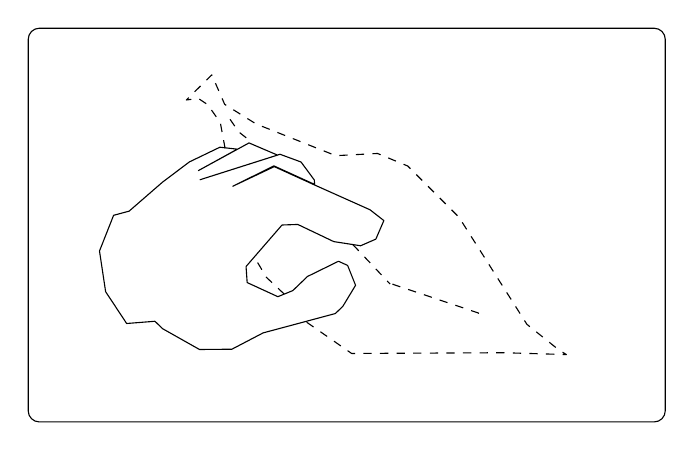
\begin{tikzpicture}
    \pgfmathsetmacro\gr{1.61803}
    \pgfmathsetmacro\by{5pt}
    \pgfmathsetmacro\bx{\by*\gr}
    \draw[rounded corners] (0,0) rectangle (\bx,\by);

    \pgfmathsetmacro\wx{1.25pt}
    \pgfmathsetmacro\wy{1.25pt}

    \draw [line join=round] (\wx,\wy) -- ++(123.46:13.784pt) -- ++(98.57:14.864pt) -- ++(68.43:13.872pt) -- ++(15:5.797pt) -- ++(40.95:16.021pt) -- ++(36.96:12.140pt) -- ++(25.73:12.210pt) -- ++(-6.34:6.339pt) -- ++(-151.16:16.059pt) -- ++(28.65:20.854pt)-- ++(-23.13:11.200pt) -- ++(-162.37:29.380pt) -- ++(17.66:30.329pt) -- ++(-20.22:8.099pt) -- ++(-53.56:8.080pt) -- ++(-86.42:1.603pt) -- ++(155.50:16.155pt) -- ++(-153.67:16.595pt) -- ++(25.33:16.595pt) -- ++(-24.50:16.155pt) -- ++(-24.10:21.800pt) -- ++(-37.95:6.341pt) -- ++(-113.40:7.301pt) -- ++(-156.43:6.001pt) -- ++(171.21:9.815pt) -- ++(154.50:14.403pt) -- ++(-177.99:5.704pt) -- ++(-130.91:19.849pt) -- ++(-86.05:5.814pt) -- ++(-24.68:12.216pt) -- ++(22.17:5.831pt) -- ++(43.90:7.355pt) -- ++(26.15:12.478pt) -- ++(-24.44:3.625pt) -- ++(-68.20:7.739pt) -- ++(-121.18:8.884pt) -- ++(-136.08:3.748pt) -- ++(-164.99:27.022pt) -- ++(-152.43:12.748pt) -- ++(-179.51:11.700pt) -- ++(150.58:15.269pt) -- ++(136.04:3.890pt) -- cycle;


    \draw [line join=round, dashed] (\wx * 2, \wy * 2.78) -- ++(100.52:9.493pt) -- ++(125.31:7.843pt) -- ++(145.78:4.031pt) -- ++(-173.09:4.432pt) -- ++(44.58:12.917pt) -- ++(-66.37:11.643pt) -- ++(-31.94:13.356pt) -- ++(-21.71:30.999pt) -- ++(3.04:15.088pt) -- ++(-22.52:11.836pt) -- ++(-45.00:26.210pt) -- ++(-57.61:45.793pt) -- ++(-38.74:14.701pt) -- ++(-31.76:3.293pt) -- ++(178.32:22.676pt) -- ++(-179.72:54.934pt) -- ++(145.20:19.950pt);

    \draw [line join=round, dashed] (\wx * 2.6, \wy * 1.3) -- ++(136.85:8.773pt) -- ++(120.74:8.3pt);

    \draw [line join=round, dashed] (\wx * 2.05, \wy * 3.075) -- ++(-55.18:5.604pt) -- ++(-38.29:4.841pt);

    \draw [line join=round, dashed] (\wx * 3.3, \wy * 1.8) -- ++(-46.66:19.524pt);

    \draw [line join=round, dashed] (\wx * 3.7, \wy * 1.4) -- ++(-18.55:32.698pt) -- ++(-45.00:.849pt);
  \end{tikzpicture}
  \caption{Heck, logical space! The hand capture those situations in which you go the supermarket, and the leaf those situations in which you obtain the ingredient.}
  \label{fig:ls:supermarket}
\end{figure}


\newpage

\section{Landscape}
\label{sec:landscape}

Weak instance: redescription.
If ends are viewed extensionally, then redescription is possible, but an agent need only reason about an end under a particular representation.
Distinguish between representations and propositions.
In the kind of scenarios, there is some representation that captures the proposition.

Slightly stronger: context.
Representations need not fully capture propositional end.
This is the kind of stuff talked about by \citeauthor{Perry:1986aa} in the case of belief.
Here, the representation is partial, but sufficient, combination with context.
Context does supplement means, as you don't have a way to establish further means to the end.

Oblique: direct reasoning fails, but you have indirect information about the end.
Cases of interest are characterised by information about means derived from the end.
There may be others.

Freudian: end constrains independent of an agent's reasoning (ends which go beyond reasoning).
In \citeauthor{Velleman:2000ab}'s terminology, it is `ungoverned by reason'.
\begin{quote}
  This flaw in the standard model is papered over, in some versions, by a characterization of desire itself as entailing the grasp of a justification for acting.
  Engagement of the agent’s rationality is thus claimed to be inherent in the very nature of desire.\nolinebreak
  \mbox{ }\hfill(\cite[9]{Velleman:2000ab})
\end{quote}
There's also an example from Russell, somewhere.
(Alternatively, Russell could be used for the first type of instance.)
Interest is in autonomous practical reasoning, but it's easier to leave this qualification implicit.
Return to the question of how to understand this divide.

\newpage


\section{The Model}
\label{sec:model}

Settling the issue of what to do doesn't require the selection of an act, it may involve the selection of multiple acts, as the information available may not be able to distinguish one act as `better' than any other act.

Think of this as a profile.
These are the acts available to you, and you rank them in some way.
The profile then settles the issue.
Can think of profiles as ranking acts, etc.
Here, think of this ranking as encoded by a probability distribution.
If the agent is uncertain about which act to perform, then there are multiple acts, and a distribution captures something like the degree to which performing the act they are confident in performing the act.
Something like this.
It's the agent's confidence in the respective action at that point in deliberation.
What deliberation gives is a way to update, this is clearest in a game theoretic setting, where there's feedback between the acts of the agent and any adversary, but the adversary isn't anything special, as long as the probability of the state of nature, so to speak, isn't fixed, then deliberation is going to be fair game.

For this kind of deliberation to make sense though, using randomness to settle the issue of what to do must be a possibility, as the way this works is to suppose that you're going to go by the distribution and then see if some other distribution would do better.
This may seem unsatisfactory, and there are questions about autonomy or whatever.


In particular, suppose we have a bounded agent, and that further reasoning is going to lead to more information about the states of nature.
See this as changes in the probability of states.




Probability distribution rather than a ranking as this allows a straightforward view of what deliberation amounts to.
It's refining this profile, which is done by revising distribution.
Here there's Jeffrey, Skyrms, Joyce, Arntzenius, etc.\
However, there's no clear consensus here.
\begin{itemize}
\item Think in terms of decision theory.
\item If you've got the decision theoretic problem, then you can find a pure strategy, at least for the specific decision --- problems in a game theoretic setting where you extend this over multiple decision --- so the probability distribution can't do better.
\item However, this only shows that the distribution is never mandated.
\item Something more is required, but at this point deliberation ends.
\item The kind of reasoning that's of interest is where deliberation is still open.
\item ``I try to plan, \dots but that isn't my basic mode, really.
  I improvise.
  It’s my greatest talent.
  I prefer situations to plans, you see \dots'' - Wintermute
\item We could try to get into the weeds here, but let's try to figure out whether the soil beneath us is fertile enough to sustain any form of life first.
\end{itemize}

Take \emph{deliberation} to capture this process.
\begin{itemize}
\item What you need is to figure out how to settle the issue.
\item What's possible and worthwhile guides you in figuring this out, but they aren't required for the issue to be settled, all that's needed for this is a profile; some determination of how to act.
\end{itemize}

\begin{itemize}
\item Whether or not this has a chance of making sense will depend on what you think the conclusion of practical reasoning is.
\item I \emph{don't} think it goes beyond the mind.
\end{itemize}

Freeze deliberation.
The decision theoretic picture makes it clear what's going on here.
Consider, by analogy, seeing someone flip a coin.
You'll update, and start to see the possibility of a bias.
They stop, and now what?
Well, the full bayesian picture will allow you to build in all your uncertainty to what you're deliberating about, so it's unclear without some further specification.
Have the tosses done enough to outweigh your priors about silver coins, do you still think it likely that your hallucinating, and so on.



Now, bootstrapping can be re-expressed in terms of taking evidence about one's deliberation, etc.\
And, the point is to deny that this is the case.
The agent has not stopped deliberating, what is given is the present state of deliberation, and this is fixed.

\newpage

\section{Further Reasoning \& Reconsideration}
\label{sec:further-reasoning-}

The core idea is that this looks a lot like the problem of reconsideration, familiar from the contemporary understanding of intention.

\begin{itemize}
\item Can the problem be reduced?
  \begin{itemize}
  \item This seems doubtful.
  \item With intentions there is an attitude, and this does a lot of the work.
  \item There may be a parallel, and this may be strengthened by arguing that in most cases the issue of further reasoning is going to be governed by some subrational process.
    However, I'm not clear on exactly how this argument should go.
    Subrational processes, sure, in the sense that most reasoning could be reduced to some subrational process, but I don't hold rationality to be \emph{that} strong, I take this to be reasoning all the same; the processing of information, and hence I don't quite understand the story of intention.
  \item This doesn't count against the reduction, then, given this understanding of what's in the `rational domain'.
  \item The bigger issue is that of an attitude.
    \begin{itemize}
    \item With intention, reconsideration is fixed by the attitude, to some degree, there's a kind of common coordinator, and it's not clear that the same holds here, in particular because this coordinator takes the attitude itself to do the work.
    \end{itemize}
  \item Well, the big distinction here is that with intention reconsideration is \emph{possible}, or at least taken to be possible, while here it is not.
  \end{itemize}
\item Is there any attitude that could do the work?
  \begin{itemize}
  \item Perhaps the ties to intentions aren't sufficiently close.
    But this doesn't rule out defining an attitude and then placing coherence constraints on this.
  \end{itemize}
\end{itemize}




\newpage



Obliqueness.
Constraint on answers to the question of what to do.
Partial information about this constraint through partial answers to the question.
Without full information about the constraint, can't be sure whether something counts as an answer.
However, partial information allows for some reasoning to take place.
In this sense, the constraint, or end, is oblique.

Two ways in which partial information helps.
\begin{enumerate*}[label=\arabic*.]
\item compatible propositions, and
\item compatible valuations of those propositions.
\end{enumerate*}
So, in the case of the shops, you can rule out propositions which don't involve obtaining an ingredient.
And, perhaps ingredients which don't align with the meal you're preparing.
Both can cause trouble.
For example, you may consider a narrow range of propositions.
If you search only for basic ingredients and what you require is partially pre-prepared.
Or, if you're following a new recipe and you rely on your valuations based on the some mistaken preconception.
Without access to the constraint to guide your reasoning, you have a harder time satisfying the constraint.
However, in the converse direction, access to a constraint does not guarantee that you will satisfy it.
Mistakes happen, and even if you aware that your end is to win a game of football, a lack of information can lead you to play cricket instead.
The broad importance of partial information is that it allows you to do some reasoning.
The issue is why the information you have counts as information.

First two scenarios were relatively straightforward.
You retained information of some broader constraint, the meal, and the need for the ingredient wasn't likely to resolve itself.
Likewise, utterances are typically quick to come and go, and if thoughtful the point you wished to make most likely still stands.
Third scenario is under-specified to the point of being opaque.
Perhaps you had been working in the study and noticed a draft, you recalled opening the window, but as you walk from your office someone closes it.
Perhaps your spouse had picked up your keys for you, or perhaps it has already been painted by your co-worker.
In these types of cases, the constraint on your reasoning has been satisfied, but without access to the constraint you do not recognise this.
Checking for drafts, patting your trousers, or looking over your contract may be natural things to do based on inclinations you have, and may indeed aid in similar scenarios, but here they have no value.

Whether or not the constraint is in place matters.
And it does so in part because of this principle:

To this need to add:
\begin{principle}\label{princip:determinable}
  \begin{itemize}
  \item Something is a candidate for settling the issue of what to do only if it can be evaluated.
  \item Something settles the issue of what to do only if it is evaluated.
  \end{itemize}

\end{principle}
Given \autoref{princip:determinable}, to settle the issue of what to does requires the processing of information.
An agent may settled what to do by arbitrary choice if their reasoning is inconclusive, but not if the choice amounts to the flip of some multi-dimensional coin.
Settling what to do is necessary for an agent to act as the result of reasoning, but not to act.


is relatively weak.
It does not state that something settling to the issue of what to do amounts to it's evaluation, and so falls short of the standard Humean principle.



These two principles together entail that when an end is oblique, reasoning premised on means to the oblique end is indeterminate.
Note, there's no contagion; it may be that if certain answers are indeterminate, then all reasoning is indeterminate, if one needs to be able to compare.
If not, then one could argue that you only need to compare to determinable answers, but then this suggests that these potential answers should be ignored.
No doubt there is some threshold, but it doesn't seem to be this.

\begin{principle}
  Something can be used to settle to the issue of what to do only if it is determinable whether or not it settles the issue.
\end{principle}
There's a better way of putting the idea here.
Something about the ability to evaluate, if you can't evaluate, then you can't figure out what information is being provided, and so you can't use it as an answer.
This kind of seems right, perhaps talk of primary value\dots
Idea is that the lack of information really is a stumbling block, and that when some information is missing, hm, some notion of `essential' information \dots
Ah, so this doesn't say anything about what makes something an answer, it just needs to be determinable, and the idea is that in these oblique cases this fails.

\begin{principle}
  Whether or not to perform an action as a means cannot be determined without being able to evaluate the end it is a means to.
\end{principle}

Answers resolve questions, but resolution is a little broader,













\newpage



Means-end reasoning answers to the question of what to do by identifying means to some end which constrains what can be done.
In this sense, means-end reasoning is narrow and contrasts with a broader sense of means-end reasoning that includes reasoning about those constraints on the question of what to do.
Perhaps there are no cases of `pure' means-end reasoning in the narrow sense.
For, it may be that there is always some way in which any potential answer to the question of what to do can be considered as a genuine answer.
The distinction is to keep track of when we can treat some end as fixed.













\newpage

Central idea is that the evaluation of options is not necessarily made on the basis of information available to an agent.

We're familiar with the idea that there may be a distinction between an agent's `true' evaluation and some ersatz evaluation that guides their practical reasoning (perhaps worth noting that ersatz can be seen as arising from failures of transparency).
For example, in cases of akrasia, weakness of will, and so on.
However, the argument here is that there doesn't even need to be a ersatz evaluation for an agent to engage in practical reasoning.
Parts of an agent's evaluation may be inaccessible but still guide an agent's reasoning.
{\color{red} (This I think is new, or fairly under-explored. The standard understanding of practical reasoning is a special case, and the more general case is kind of interesting.)}

On the logic side, develop a formalism to capture the background structure.
This doesn't account for the specific reasoning, but it does something to set up a framework for explaining the basic principles and suggesting how the basic idea can be extend to decision theoretic contexts, etc.


This doesn't directly reduce to a kind of cognitivism, though it comes close.
Roughly, if cognitivism holds, then the central thing is belief about what's `good', and one can view this all in terms of a cognitivist structure, in which one's means are providing evidence of a kind, but I don't think it follows that this is the way to do the work.
Rather, it's a familiar gloss.
But, you need more to get the cognitivist picture going\dots
Unless, of course, the picture is that cognitivist just amounts to there being reasoning involved, and hence in contrast to a kind of struct Humean position.

Perhaps useful to contrast Broome's ``core type'' of reasoning in `Rationality through reasoning', as this involves language of a kind, etc.

Reflection principles!


\section{Notes on the interpretation}
\label{sec:notes-interpretation}

Here, the basic idea is that there's some kind of evaluative function that's specifying beliefs and desires, and the modal is picking up something of a threshold.
This can be seen as binary, etc.\ but the important thing is that there's nothing to special about the set of situations.
Either these are those for which the valuation is `true', or there's some relevant threshold, etc.\ but more generally the same evaluative principle can be applied to other states, and with this I can reason about means, ends, and the like from the perspective of desires, beliefs, and more.
It's in this sense that these are propositional attitudes.
Again, this goes back to the idea of tests, which I don't think fits into the broad picture that I'm trying to motivate here, but \dots

This probably contrasts to the \(O\phi \coloneq G \rightarrow \phi\) approach, as here there's an explicit proposition that's the good, and it's the logical relation this has to other states which is important.
So, no propositional attitude, at least on a fairly natural interpretation.


\section{Notes on the formalism}
\label{sec:notes-formalism}

Failure of cloaure under negation for the oblique fragment, and closing under negation as the way to figure out the recognised situations.
However, this means that I don't have an \emph{abstract modal logic} in the blue books sense of the term (p.\  476).
But temporal logic ain't an abstract modal logic, so this failure isn't too interesting.

`The best introduction to expressive completeness is the encyclopedic Gabbay, Hodkinson, and Reynolds [163]; both separability and game-based proofs are discussed. It also contains many other results on since and until logic and a useful bibliography.'

Possibly easier to axiomatise what's going on by using a kind of global modality.
This is inspired by \citeauthor{van-Benthem:1979aa}'s ideas about Leibniz's ideas of permissibility and so on.
However, on \citeauthor{van-Benthem:1979aa}'s approach, there's a modality picking up on the accessible worlds, whereas with what I'm interested in, I want the accessibility relation to be genuinely global.
This, is likely a problem.
Oh, following the blue book, the global modality alone has a decidable satisfiability problem.
The axiomatisation is seemingly simple too, with the standard S5 axioms being supplemented with \emph{inclusion}:
\[\Diamond p \rightarrow E\phi\]
Where \(Ep\) means that there's some \(p\) world in the model.
And, this apparently applies to normal modal logics quite generally.
Interesting that this global modality can't define irreflexivity.
If permissibility is able to do this, then there are probably questions about decidability.

From Gargov, Passy, Tinchev, it looks as though standard canonical model type constructions can be used to prove completeness for the box and window logic.
And, I have a feeling this should also work for partial logic.
A difficulty might be in generating MCSs, but here maybe either treat negations properly, or introduce an additional syntactic component to identify lack of truth value.
I mean, in a sense these aren't going to be MCSs, as adding some atomic expression would likely preserve consistency, while also violating the idea that arbitrary atomic expressions can be undefined.

\begin{enumerate}
\item \(\attn{\phi} \rightarrow \phi\), to ensure appropriate subset relation.
\end{enumerate}

I think this is the only thing required.
And, the reason to be interested in MCSs is to ensure one considers every `possible world'.
This is useful for finding counterexamples.
An additional syntactic component to capture undefinedness should be fine.
The partial operator(s) may be a little more difficult, but this isn't obvious.



\newpage

A stack of articles is at rest on my desk.
The yellow post-it note stating ``for research idea'' indicates that the stack was put to rest.
Some time ago I fixed some end, some research idea, and the articles were assembled as means to that end.
Some thing interrupted my performance of the means, and I can not now recall the idea to which the articles were a means to pursuing.
However, the organisation of the stack and light annotation to some pages suggest I may be able to recall the research idea by working through the stack.

My reasoning about whether to read the articles is an instance of mundane scenarios in which the instrumentalist means-end structure of practical reasoning is inverted.
In these scenarios, an agent recognises means to some end, but does not have the resources to reason about the end.
And, in turn, the agent recognises that their present evaluation of the means may diverge from their evaluation of the means were they to have to the resources to reason about the end.
Without the ability to reason about the research idea, I lack the ability to appropriately evaluate working through the stack.
For, were I able to reason about the research idea that the stack of papers were a means to, I would be able to evaluate the idea and in turn of whether to work through the stack.
If were to no longer view the idea as viable it may be that I should pursue some other activity, while if I still regard the idea as viable I have an activity set out for me.

Let us term this end-means reasoning.
End-means reasoning is not the strict inverse of standard means-end reasoning.
For, means-end reasoning typically proceeds from some recognised end to recognised means, while end-means reasoning requires some representational lacuna.
The stack of articles were a means to finding something sensible to say about cases of end-means reasoning, working through the stack was valuable given this end, and I reasoned that this end was worthwhile pursuing despite my inability to reason about it directly.
And, we are here because I was successful in reconstructing the end after pursuing the means to it.

What I have to say about end-means reasoning is fairly straightforward.
We are agents with bounded resources, and some of these bounds relate to the possibilities we are able to reason about.
Cases of end-means reasoning arise when changes in our representational resources lead to the inability to recognise possibilities that was previously identified as an end, though the resources required to represent chosen means toward that end persist.
This lack of representational resources then indicates to the agent that the evaluative judgements they can make may diverge from those they would make given additional representational resources, but their recognition of the specified means as means allows them to indirectly reason about the evaluative judgements they may make given additional representational resources.\nolinebreak
\footnote{TODO: Simplify this! The key point is that the agent's practical reasoning isn't premised on their current evaluative judgements.
  In this respect, the issue is very similar to the way I've been thinking about cases of temptation.
  An agent attempts to reason about what their `more refined' evaluative judgements would be.
  This is also super close to what Smith does with ideal advisers, but without the ideal part (and I think for a fairly different application).
}

In this respect, end-means reasoning is an instance of \emph{oblique} reasoning; reasoning which goes beyond the representational resources that you have at your disposal.
\begin{center}
  [More to say here\dots]
\end{center}

The goal is to make this sketch into a precise analysis.
In doing so I hope to show that cases of end-means reasoning can complement whatever your understanding of practical reasoning is.
In turn, I hope that your understanding of practical reasoning helps shed light on normative and descriptive aspects of end-means reasoning.
This assumes that your understanding of practical reasoning does not rule out the possibility of end-means reasoning, but beyond this the specific account of end-means reasoning I give is meant to be illustrative.
The analysis is framed in terms of more-or-less well explored formal treatments of folk theory.
I will explain and augment this framework as required, but I expect you to translate the analysis to any other framework as you see fit.


Aim to show some degree of continuity!


\begin{center}
  [\textbf{Structure of the paper.}]
\end{center}

\newpage

The important idea with these types of cases isn't the way reasoning is structured, but how ends function, I think.
In that, with the record store case, the supermarket case, and so on, the broad instrumentalist picture of practical reasoning can be preserved.
The end is still fixed, and so you can have the `end' of completing the means, but this won't have much actionable content.
The thing is that this isn't really a new end, rather this is a redescription of the same end, and something like this is always going to be possible with the kind of cases I've set up.
Hence, the claim that the reasoning is different is due to the relative importance of the means, etc.
In standard cases, you can always reevaluate the means with respect to the end that they're a means to, whereas here, there's no way to figure out whether they should be developed/reformed etc.

What's important, is that there's no straightforward way to evaluate the actions compatible with your means.
In this respect, the relevant reasoning can't be weighing up reasons for an against, etc.\ because there's no way to recognise those reasons, speaking loosely.
Similarly, perceived desirability and so on seem problematic.
From a different point of view, there's some full evaluation function, and the agent only has restricted access to it.

So, an idea is that this is a special case of weakness/strength of the will.
For, in these cases the desirability of the means may drop below the desirability of other courses of action.
However, you see that there's something missing in your evaluation, and you may still pursue the means.

In terms of reasons, there's the contrast between considering all of the reasons for and against an action, and considering those which are `available' to you.
And, in the cases I'm thinking of, you're not interested in all the reasons for and against, but you're still interested in reasons which go beyond what are available to you.

In part, this is because the reasons that are no longer available to you did impact your evaluation of actions, and you still have some information about this.

So, the general perspective on practical reasoning that I want to pursue here is one in which evaluative judgements are foundational but do not exhaust practical reasoning.
And, approaching this from the perspective of propositional attitudes gives something very coarse grained.
It allows one to kind of see how the partiality is functioning, but if the relevant judgements rely on any kind of comparative notion, then the model won't have the resources to capture this.
Exploring the more fine grained comparisons doesn't look too straightforward, either.
One way of doing this, though, would be to assume that there's an evaluative function on situations.
For if this is the case, then the evaluation of complex expressions can be treated compositionally, and hence a more fine grained evaluation can be tied to a partial denotation.

With these examples, what needs to be stressed is that you're not relying on your current evaluative judgement regarding the means that you have selected.
Rather, you're relying on some other evaluative judgement.
Hence, there's some kind of end-means reasoning, in terms of how one's evaluative judgements are being formed.
Usually, the evaluation of means proceeds from the evaluation of ends, but here it's almost the other way round.

% Due to the means-end structure of the relevant reasoning here, it's not clear that this straightforwardly hooks up to issues about incomplete preferences.
% For, on my understanding, this primarily concerns how to make evaluative judgements, whereas here it seems as though no explicit evaluative judgement is required, or going to be of any substantial help, as the appropriate evaluation of the options available to you is there, but inaccessible.

% The way I'm thinking about means and ends seems to be close to how \citeauthor{Bratman:1987aa} thinks about intentions.
% Roughly, the specification of an end narrows down one's desires, but this isn't given by one's desires, etc.\ so it can't simply be a mental state on par with desire.



\newpage

\section{Formalism}
\label{sec:formalism}

Two things we need to capture.
Our theoretical perspective and the agent's perspective.

Standard treatment of propositional attitudes.
Collections of situations.

\begin{definition}[Frame]
  A \emph{frame} \(\oframe{F}\) is a pair \((S,\langle A_{1},\dots,A_{n} \rangle)\) where
  \begin{itemize}
  \item \(S\) is a collection of points capturing situations,
  \item Each \(\fatt{} \colon S \to \wp(S)\) is a function associating to each situation a subset of situations which are compatible with the agent's attitde.
  \end{itemize}
  Attitudes may satisfy certain requirements, e.g.\ if \(t \in \fatt{u}\) then \(\fatt{t} = \fatt{u}\), etc.
  However, we do no assume this.
  In this respect, attitudes can be treated as standard relations.
\end{definition}
A frame can be augmented to include further distinguished subsets, and multiple distinguished subsets corresponding to multiple agents may be intruded.
Frames fix the situations and what the agent `desires' and `believes' independently of the resources we have to reason about these.
{\color{red} This should be reformulated.
  What's required here are `desire-like' and `belief-like' attitudes.
  The former can the correspond to desires, ends, and the like, while the latter to beliefs, means, and the like.
  And, frames should permit (at least) finite collections of these.}

\emph{Expressions} builts from some langauge are used to talk about a frame, and our primary interest will be in the \emph{propositions}, or collections of situations, that expressions refer to.
Key to our understanding of oblique attitudes is capturing the appropriate expressive power of a language with respect a frame, but nothing rests on our use of the terms `proposition' and `expression' other than this distinction between aspects of a language and their interpretation.

\begin{definition}[Propositions]
  Subsets of the collection of situations.
  Specified with respect to a frame.
\end{definition}

\begin{definition}[Atomic Expressions]
  Set of symbols \(\mathsf{Exp}\), non-logical.
\end{definition}

Every expression denotes a proposition, but it does not follow that for every proposition there is a corresponding atomic expression.
Resources are captured via interpreting the frame through expressions which denote collections of situations.
Hence, agents aren't necessarily able to reason about arbitrary collections of sitations.
Instead, the agent has expressions, and their reasoning is bounded by the collections of situations that these refer to.
And, there's no guarantee that any given collection of sitatuations is characterised by an expression.
While we have only introduced atomic expressions, this claim extends to arbitrary expressions, detailed below.

Propositional attitutdes are understood with respect to this characterisation of propositions.
Hence, for an agent to have an attitude toward a proposition is not for an agent to have an attitude toward an expression.
Rather, for an agent to have an attitude toward a proposition is for there to be a relation between an agent and a collection of sitautions.
In turn, this is a coarse grained perspective on the functional profile of an agent.
For example, the \emph{beliefs} of an agent are captured through the proposition corresponding to the situations they are unable to distinguish from the actual situations.
The \emph{desires} of an agent are captured by collecting the situations in which they would be satisfied.
Likewise, the \emph{means} and \emph{ends} adopted by an agent may be characterised through compatible situations.



Rare that an agent will identify a unique sitaution.
Indeed, if an agent can uniquely identify each sitaution, then they may be able to reason about arbitrary propositions.
In part this captures bounded resources.
Though, this aspect of bounded agency is captured quite generally, whether it is made explicit or not.\nolinebreak
\footnote{Indeed, it follows from some natural formal constraints.
  For, given an infinite set of situations, there are uncountably many collections of situations, and languages are typically restricted to countably many expressions.}
Primary sense of a resource is being able to put a proposition to some use.
Expressions, then, amount to resources, as do the attitudes specified at the frame level.

To capture reasoning regarding oblique attitudes we separate two distinct ways a given atomic expression can be put to use by an agent.

First, there is the \emph{support} that an expression gives to an agent's reasoning.
The support of an expression identifies those situations which are compatible with the expression and those which are incompatible with the expression.\nolinebreak
\footnote{We use the terms `compatible' and `incompatible' as generic placeholders.
  For, while we assume that the support of an expression amounts to the truth conditions of an expression, this is merely a simplifying assumption.
  Gaps and gluts may inform the backdrop of an agent's reasoning, but these are potential complications that we set aside at present.}
Second, there is the \emph{application} of an expression in an agent's reasoning.
These are the situations that an agent takes to be compatible and incompatible with the expression.

Key to our analysis is the idea that an agent's reasoning may only apply to a subset of the situations supported by an expression.
In this respect, an agent's application of an expression may be \emph{partial}.

\begin{center}
  [Explanation of examples]
\end{center}

\begin{figure}[ht]
  \centering
  \begin{subfigure}[b]{0.3\textwidth}
    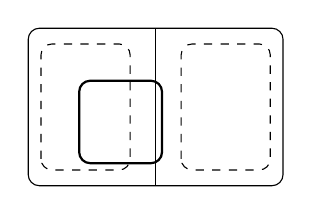
\begin{tikzpicture}
      \pgfmathsetmacro\gr{1.61803}
      \pgfmathsetmacro\by{2}
      \pgfmathsetmacro\bx{\by*\gr}
      \draw[rounded corners] (0,0) rectangle (\bx,\by);

      \draw (\bx/2,0) -- (\bx/2,\by); % Centre division

      \draw[rounded corners, thick] (\bx*0.2, \by/1.5) rectangle (\bx*0.525,\by/7);

      \draw[rounded corners, dashed] (\bx*0.05, \by*0.1) rectangle (\bx*0.4,\by*0.9);
      \draw[rounded corners, dashed] (\bx*0.6, \by*0.1) rectangle (\bx*0.95,\by*0.9);
    \end{tikzpicture}
    \caption{}
  \end{subfigure}
  \begin{subfigure}[b]{0.3\textwidth}
    \centering
    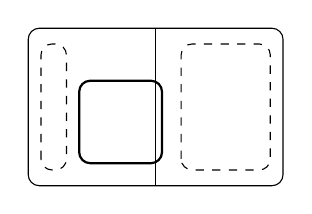
\begin{tikzpicture}
      \pgfmathsetmacro\gr{1.61803}
      \pgfmathsetmacro\by{2}
      \pgfmathsetmacro\bx{\by*\gr}
      \draw[rounded corners] (0,0) rectangle (\bx,\by);

      \draw (\bx/2,0) -- (\bx/2,\by); % Centre division

      \draw[rounded corners, thick] (\bx*0.2, \by/1.5) rectangle (\bx*0.525,\by/7);

      \draw[rounded corners, dashed] (\bx*0.05, \by*0.1) rectangle (\bx*0.15,\by*0.9);
      \draw[rounded corners, dashed] (\bx*0.6, \by*0.1) rectangle (\bx*0.95,\by*0.9);
    \end{tikzpicture}
    \caption{}
  \end{subfigure}
  \begin{subfigure}[b]{0.3\textwidth}
    \centering
    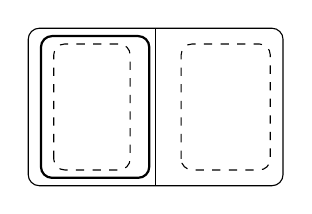
\begin{tikzpicture}
      \pgfmathsetmacro\gr{1.61803}
      \pgfmathsetmacro\by{2}
      \pgfmathsetmacro\bx{\by*\gr}
      \draw[rounded corners] (0,0) rectangle (\bx,\by);

      \draw (\bx/2,0) -- (\bx/2,\by); % Centre division

      \draw[rounded corners, thick] (\bx*0.05, \by*0.05) rectangle (\bx*0.475,\by*0.95);

      \draw[rounded corners, dashed] (\bx*0.1, \by*0.1) rectangle (\bx*0.4,\by*0.9);
      \draw[rounded corners, dashed] (\bx*0.6, \by*0.1) rectangle (\bx*0.95,\by*0.9);
    \end{tikzpicture}
    \caption{}
  \end{subfigure}
  \caption{Application examples}
\end{figure}

From a formal point of view, the support and application of an expression are both instances of what we term a \emph{denotation}; a pair of functions mapping an atomic expression to those compatible and incompatible situations, respectively.

\begin{definition}[Denotation]
  Given a frame \(\oframe{F}\) and set of atomic expressions \(\atmexp\), a \emph{denotation}, \(D = \langle \cdeno{},\ideno{} \rangle\), is a pair of functions
  \begin{align*}
    \cdeno{} \colon \mathsf{Exp} \to \wp(S) & & \ideno{} \colon \mathsf{Exp} \to \wp(S)
  \end{align*}
  such that for every \(P \in \mathsf{Exp}, \cdeno{P} \cap \ideno{P} = \emptyset\).

  If for every \(P \in \mathsf{Exp}\) we have \(\cdeno{P} \cup \ideno{P} = S\), then we call the denotation \emph{full}.\newline
  Else, we call the denotation \emph{partial}.
\end{definition}

Given two denotations \(D_{1} = \langle \cdeno[d_{1}]{},\ideno[d_{1}]{} \rangle\) and \(D_{2} = \langle \cdeno[d_{2}]{},\ideno[d_{2}]{} \rangle\), if for all \(P \in \mathsf{Exp}\),
\begin{enumerate*}[label=]
\item \(\cdeno[d_{1}]{P} \subseteq \cdeno[d_{2}]{P}\) and
\item \(\ideno[d_{1}]{P} \subseteq \ideno[d_{2}]{P}\),
\end{enumerate*}
then we say that \(D_{1}\) is a \emph{restriction} of \(D_{2}\) or, conversely, that \(D_{2}\) is an \emph{expansion} of \(D_{1}\).

Full denotation can be taken to correspond to truth conditions.
This is the intended perspective.
Application is then the way the agent applies these truth conditions.
However, this can be seen as an idealising assumption that one may not want to make.
Allowing an agent to diverge can be useful.





To \emph{interpret} a collection of atomic expressions with respect to some frame, then, we require a pair of related denotations.
First a full denotation to capture to the support of any atomic expression and second a potentially partial denotation to capture its application.

\begin{definition}[Interpretation]
  Given a collection of atomic expression \(\mathsf{Exp}\) and a frame \(\oframe{F}\), an interpretation, \(\mathcal{I} = \langle \mathcal{S},\mathcal{A} \rangle\), is a pair of denotations where \(\mathcal{A}\) may be partial denotation and \(\mathcal{S}\) is a full denotation expanding \(\mathcal{A}\).
\end{definition}

{\color{red} Intuitively, \dots this means that we can treat \(\mathcal{S}\) as providing truth conditions and \(\mathcal{A}\) as providing an agent's application of these truth conditions.}

Given a collection of atomic expressions, a frame paired with an interpretation forms a model.

\begin{definition}[Model]
  An \emph{oblique model} \(\omodel{M} = \langle \oframe{F}, \ointp{I} \rangle\) is a frame together with an interpretation.
\end{definition}

Given a scenario, the specification of a model captures core aspects of the phenomena we are interested in.
For, we can state what beliefs and desires an agent has, we can then study how atomic expressions relate to an agent's beliefs and desires, the relations which hold between atomic expressions, and the result of composing atomic expressions to form complex expressions.
As in the examples above, natural language is adequate for this task.
%TODO Maybe say more here
Still, introducing a formal language affords us an easier investigation of complex models and helps fix the foundation for a systematic study of models in general.

The logical language we use to reason about complex expressions, interplay between the support and application of expressions, and the desires and beliefs of agents is a generalisation of the basic modal language.
We include the standard logical operations of negation and conjunction, two modalities to capture the desires and beliefs of the agent, and two additional \emph{oblique} operators to reason about the application of expressions by an agent.

\begin{definition}[Oblique language]
  Given a collection of atomic expressions \(\mathsf{Exp}\), the well-formed expressions \(\phi\) of an \emph{oblique language} \(\olang{}\) are given by the following rule:
  \[
    \phi \Coloneqq P \in \mathsf{Exp} \bnfsep \lnot\phi \bnfsep \phi\land\psi \bnfsep \phi\lor\psi \bnfsep \lattu[A_{i}]{\phi} \bnfsep \lattd[A_{i}]{\phi} \bnfsep \attn{\phi} \bnfsep \phi \ltrans \psi
  \]
\end{definition}

Given that an interpretation of a frame consists of two denotation functions which are themselves pairs, the way in which we understand expression in given oblique language requires some care.
First, we shall treat expressions as referring to the situations they are compatible with, and use negation of an expression (\(\lnot\)) to refer to those situations incompatible with the expression.
Second, we will default to taking an expression to refer to its support.
The unary operator \(\attn{\cdot}\) is then given to indicate the application of an expression.\nolinebreak
\footnote{Either we must fix our understanding of an expression relative to a denotation, or we must provide a way to switch from one denotation to another.
  Either option is viable, but we chose the latter as this affords us the ability to mix the support and application of an expression when building complex expressions.
This ability is useful to have, as we can the express relations which hold between our perspective and the agents.}

For example, \(P\) is be read as referring to the situations which are compatible with the support of \(P\), while \(\attn{P}\) is read as referring to the situations compatible with the application of \(P\).
Complex expressions may combine both support and application.
Hence, \(P \land \attn{\lnot Q}\) will refer to the situations which are compatible with the support of \(P\) and are incompatible with the application of \(Q\).

The binary operator \(\cdot \ltrans \cdot\) serves as a restrictor of sorts.
The expression \(\phi \ltrans \psi\), reads `\(\phi\) is compatible with all the situations compatible with \(\psi\)'.
\(\attn{\phi} \ltrans \phi\) will always hold, as the application of \(\phi\) always denotes a subset of the support of \(\phi\), however \(\phi \ltrans \attn{\phi}\) may not hold, as an agent may fail to consider some \(\phi\) situations in their application of the expression.

\begin{figure}[ht]
  \centering
  \begin{subfigure}[b]{0.4\textwidth}
    \centering
    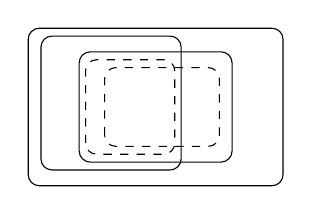
\begin{tikzpicture}
      \pgfmathsetmacro\gr{1.61803}
      \pgfmathsetmacro\by{2}
      \pgfmathsetmacro\bx{\by*\gr}
      \draw[rounded corners] (0,0) rectangle (\bx,\by);

      \draw[rounded corners] (\bx*0.05, \by*0.1) rectangle (\bx*0.6,\by*0.95);

      \draw[rounded corners, dashed] (\bx*0.225,\by*0.2) rectangle (\bx*0.575,\by*0.8);

      \draw[rounded corners] (\bx*0.2, \by*0.15) rectangle (\bx*0.8,\by*0.85);

      \draw[rounded corners, dashed] (\bx*0.3,\by*0.25) rectangle (\bx*0.75,\by*0.75);
    \end{tikzpicture}
    \caption{\(Q \ltrans \attn{P}\), \(\sim(Q \ltrans P)\)}
  \end{subfigure}
  \begin{subfigure}[b]{0.4\textwidth}
    \centering
    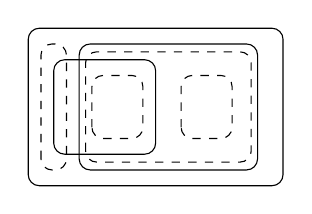
\begin{tikzpicture}
      \pgfmathsetmacro\gr{1.61803}
      \pgfmathsetmacro\by{2}
      \pgfmathsetmacro\bx{\by*\gr}
      \draw[rounded corners] (0,0) rectangle (\bx,\by);

      \draw[rounded corners] (\bx*0.1, \by*0.2) rectangle (\bx*0.5,\by*0.8); % P
      \draw[rounded corners] (\bx*0.2, \by*0.1) rectangle (\bx*0.9,\by*0.9); % Q

      \draw[rounded corners, dashed] (\bx*0.05, \by*0.1) rectangle (\bx*0.15,\by*0.9); % a~Q
      \draw[rounded corners, dashed] (\bx*0.225, \by*0.15) rectangle (\bx*0.875,\by*0.85); % aQ
      \draw[rounded corners, dashed] (\bx*0.6, \by*0.3) rectangle (\bx*0.8,\by*0.7); % a~P
      \draw[rounded corners, dashed] (\bx*0.25, \by*0.3) rectangle (\bx*0.45,\by*0.7); % aP
    \end{tikzpicture}
    \caption{\(\attn{Q}\ltrans\attn{P}, \attn{Q}\ltrans\attn{\lnot P}\)}
  \end{subfigure}
  \caption{Examples of transplication}
\end{figure}

A note on negation.
Restriction restricts to those situations compatible.
So, reference is determined by restrictor.
This means that \(\lnot \phi \ltrans \psi\) is equivalent to \(\lnot(\phi \ltrans \psi)\).
In other words, the restrictor always takes wide scope.
Because the reference of the expression is determined by the restriction.
To express the fact that something doesn't follow from a restriction, we can simply express the consistency of the restriction and the negation of that thing.
So, \(\lnot\bot \ltrans (\lnot \phi \land \psi)\).




The semantic relationship between the support and application of an expression requires some subtlety in our construction of an interpretation function.
We begin by defining the \emph{exclusive fragment} of an oblique language.
This consists of those expressions built from a set of atomic expressions and simple logical operators.

\begin{definition}[Exclusive fragment of an oblique language]
  Given a collection of atomic expressions \(\mathsf{Exp}\), the \emph{exclusive} well-formed expressions \(\phi\) of an oblique language \(\olang{}\) are given by the following rule:
  \[
    \phi \Coloneqq P \in \mathsf{Exp} \bnfsep \lnot\phi \bnfsep \phi\land\psi \bnfsep \phi\lor\psi \bnfsep \phi \ltrans \psi
  \]
\end{definition}

The simplicity of this fragment of the oblique language is due to the fact that the denotation of these expressions are straightforwardly given from the denotation of their sub-expressions.
In other words, the denotation of any expression built from the exclusive fragment of an oblique language corresponds to either the support or the application of the expression, and hence can be specified by a single denotation.

\begin{definition}[Denotation of exclusive oblique expressions]
  Given an oblique frame \(\oframe{F}\), a set of atomic expressions \(\atmexp\), and denotation \(D = \langle \cdeno{}, \ideno{} \rangle\), \(D\) extends to the exclusive fragment of  \(\olang{}\) in the following way.
  \begin{align*}
    \cdeno{\lnot\phi} &= \ideno{\phi} & \ideno{\lnot\phi} &= \cdeno{\phi} \\
    \cdeno{\phi \land \psi} &= \cdeno{\phi} \cap \cdeno{\psi} & \ideno{\phi \land \psi} &= \ideno{\phi} \cup \ideno{\psi}  \\
    \cdeno{\phi \lor \psi} &= \cdeno{\phi} \cup \cdeno{\psi} & \ideno{\phi \lor \psi} &= \ideno{\phi} \cap \ideno{\psi} \\
    \cdeno{\phi \ltrans \psi} &= \cdeno{\psi} \cap \cdeno{\phi} & \ideno{\phi \ltrans \psi} &= \cdeno{\psi} \cap \ideno{\phi} \\
    \cdeno{\lattu{\phi}} &= \{s \in S \mid \fatt{s} \subseteq \cdeno{\phi}\} & \ideno{\lattu{\phi}} &= \{s \in S \mid \fatt{s} \cap \ideno{\phi} \ne \emptyset\}\\
    \cdeno{\lattd{\phi}} &= \{s \in S \mid  \fatt{s} \subseteq \ideno{\phi}\} & \ideno{\lattd{\phi}} &= \{s \in S \mid \cdeno{\phi} \nsubseteq \fatt{s}\}\\
  \end{align*}
\end{definition}

The key thing about complex expressions is that they are built using logical vocabularly, and hence are compositional.
So, for a given snapshot we have a way to interpret expressions.
From the theoretical standpoint, compositional operators are tools which allow us to refer to those propositions which can be constructed from more basic propositions.

What usually goes under the heading of `truth fuctional completeness' ensures that the operators allow us to capture any relevant construction.
The same holds for a partial interpretation, {\color{red} so long as we're interested in monotonic operators}.

From the perspective of understanding an agent's application of an expression, it may seem that we are endowing the agent with a kind of logical omniscience.
There are two sense of this.
First, not limit on the expressions available to an agent.
Second, no possibility of application being non-compositional.

First, we're capturing are the resources available to an agent, an available here is in a weak sense.
Second, non-compositionality would be a significant increase to complexity.
So, idealising, but also we'd want to be able to capture what the agent could do with their resources.
Hence, this idealisation is best seen as a conflation of two things.

Still, this is a foundation, rather than a complete framework.
Hence, we can informally specify what the agent recognises, and we can introduce atomic surrogates for complex expressions.
For example \(p `\land' q\) such that \(p `\land' q \rightarrow p[q]\), etc. 


Connexion to partial logic.

\begin{fact}
  \(\ideno{\phi \ltrans \psi} \ne \emptyset\) iff \(\cdeno{\lnot\bot \ltrans (\lnot\phi \land \psi)} \ne \emptyset\).
  \begin{proof}
    \(\ideno{\phi \ltrans \psi} \ne \emptyset\) iff \(\ideno{\phi} \cap \cdeno{\psi} \ne \emptyset\) iff \(\cdeno{\lnot\phi} \cap \cdeno{\psi} \ne \emptyset\) iff \(\cdeno{\lnot\phi \land \psi} \ne \emptyset\) iff \(\cdeno{\lnot\bot} \cap \cdeno{\lnot\phi \land \psi} \ne \emptyset\)
  \end{proof}
\end{fact}

An \emph{interpretation} of an oblique language is a straightforward combination of two denotations.

\begin{definition}
  Given a frame \(\mathfrak{F}\), an interpretation \(\Intp\) of a collection of atomic expressions \(\mathsf{Exp}\) applies to a language \(\mathcal{L}\) built from those same expressions in the following way.
  \begin{align*}
    \cintp{P} &= \csupp{P} & \iintp{P} &= \isupp{P}\\
    \cintp{\lnot\phi} &= \iintp{\phi} & \iintp{\lnot\phi} &= \cintp{\phi}\\
    \cintp{\phi \land \psi} &= \cintp{\phi} \cap \cintp{\psi} & \iintp{\phi \land \psi} &= \iintp{\phi} \cup \iintp{\psi}\\
    \cintp{\phi \lor \psi} &= \cintp{\phi} \cup \cintp{\psi} & \iintp{\phi \lor \psi} &= \iintp{\phi} \cap \iintp{\psi}\\
    \cintp{\phi \ltrans \psi} &= \cintp{\psi} \cap \cintp{\phi} &  \iintp{\phi \ltrans \psi} &= \cintp{\psi} \cap \iintp{\phi}\\
    \cintp{\lattu{\phi}} &= \{s \in S \mid \fatt{s} \subseteq \cintp{\phi}\} & \iintp{\lattu{\phi}} &= \{s \in S \mid \fatt{s} \cap \iintp{\phi} \ne \emptyset\}\\
    \cintp{\lattd{\phi}} &= \{s \in S \mid  \fatt{s} \subseteq \iintp{\phi}\} & \iintp{\lattd{\phi}} &= \{s \in S \mid \cintp{\phi} \nsubseteq \fatt{s}\}\\
    \cintp{\attn{\phi}} &= \cappl{\phi} & \iintp{\attn{\phi}} &= \iappl{\phi}\\
  \end{align*}
\end{definition}


\begin{proposition}
  The semantic clauses for \(\Box\) and \(\Window\) on relational models are as follows:
  \begin{enumerate}
  \item \(M,s \vDash \Box\phi\) iff \(\forall t(Rst \Rightarrow M,t \vDash \phi)\)
  \item \(M,s \Dashv \Box\phi\) iff \(\exists t(Rst \land M,t \Dashv \phi)\)
  \item \(M,s \vDash \Diamond\phi\) iff \(\exists t(Rst \land M,t \vDash \phi)\)
  \item \(M,s \vDash \Window\phi\) iff \(\forall t(\lnot Rst \Rightarrow M,t \Dashv \phi)\)
  \item \(M,s \Dashv \Window\phi\) iff \(\exists t(\lnot Rst \land M,t \vDash \phi)\)
  \item \(M,s \vDash \Kite\phi\) iff \(\exists t(\lnot Rst \land M,t \Dashv \phi)\)
  \end{enumerate}

\end{proposition}

Note, here there's no difference between the support and the application of any propositional attitude.
This is a simplification, and we could revise the definition of an interpretation to allow for variation.
This would amount to revising the notion of a denotation to allow for weaker conditions on attitudes.
For, these are not straightforwardly given by more basic expressions.
And, as we're not too interested in issues arising from iterated attitudes, the added complexity is avoided.


\begin{note}
  Propositional attitudes.
  These are of interest for us as theorists.
  However, their interpretation is based in capturing information available to the agent.
  \(\lattu{\phi}\) states that every state the agent considers is a \(\phi\) state, while \(\lnot\lattu{\lnot\phi}\) captures the fact that the agent recognises that there is a state where \(\phi\) does not hold.
  Note, this means that if both \(\phi\) and \(\lnot\phi\) fail to hold, then neither \(\lattu{\phi}\) nor \(\lnot\lattu{\lnot\phi}\) will hold.
  So, as theorists we must rely on metalinguistic statements to capture the fact that an agent fails to consider a proposition.

  Alternatively, we may introduce a complementary operator to fill in the gap.
  This operator, however, would not be monotonic.
  Capturing the monotonic core is useful, as states are partial only with respect to the agent's reasoning.
  Hence, any monotonic inferences will hold regardless of how the agent's information develops.
  `Valid' inferences here, then, will hold unless there are changes to the agent's attitudes.
  Of course, changes to the agent's attitudes are what we're interested in, but a clean separation between the two cases is useful to have.

  This is the reason for the perhaps unintuitive downward operator.
  However, non-monotonic operators are no better than diamond modalities, when it comes to partial states which may be refined.
  In certain respects, then, this requires the agent to be aware that they only have a partial representation of the possibilities.
\end{note}



Belief and desires should be noted.
As, the interpretation of these is fixed by the language, but is only specified with respect to the interpretation.
The basic idea is that our interest in propositional attitudes is as a theorist.
And, for the present purposes we're not interested in higher order attitudes.
So, while iteration isn't prohibited, we do not take these to constitute resources available to an agent.

Else, we should extend denotations to cover these, and this is a lot.
First, different application for support and application of prejacent(?).
Second, problem of specifying complex formulas.

\begin{definition}[Support]
  \(M,X \vDash \phi\) iff \(X \cap (\cintp{\phi} \cup \iintp{\phi}) \subseteq \cintp{\phi}\).

  Hence, \(M,X \vDash \phi\) iff \(X \cap \iintp{\phi} = \emptyset\).

  If \(X = \{s\}\), we write \(M,s \vDash \phi\).

  \(M,s \vDash \lattu{\phi}\) iff \(\fatt{s} \cap (\cintp{\phi} \cup \iintp{\phi}) \subseteq \cintp{\phi}\) iff \(M,\fatt{s} \cap (\cintp{\phi} \cup \iintp{\phi}) \vDash \phi\).
\end{definition}

Atttiudes of agents towards expressions are viewed as providing additional valuations to expressions.
Natural language, ``\(\phi\) is desirable'' suggests that a certain perspective is taken toward \(\phi\) by the agent.
However, this is the result of some valuation of situations.
In general, expressions and an agent's application of expressions may be indpendent of the way in which situations interact with an agents reasoning.
Governing principle is that attitudes concern collection of situations, not expressions.
This is why terminology of propositional attitudes is adopted.
The reltaionship between propositional attitudes and expression can be seen as the composition of two operations.
First, consider the states evaluated by the attitude, and second determine the relation that an expression bears to them.

The relationship between the proposition and the expression can then be put to different uses.

Familiar notion of an expression being entailed by a proposition.
This captures a form necessity.
Foundation of our understanding of doxastic states.
For an expression to capture belief, it must be the case that the expression holds in all epistemically possible worlds.
With desire-like attitudes this remains important, as we have an account of what is required for a desire to be satisfied, but sufficiency is also key.
Sufficiency is stronger than mere consistency.
For, consistency states that one way of \(\phi\) obtaining would be satisfactory, while sufficiency states that any way of \(\phi\) working out would be satisfactory.

Attitudes concern collections of situations, not expressions.
Collections of situations can only be reasoned about through expressions.
Hence, agent's only have indirect access to their own atittudes.







Two types of opeators used to captures attitudes of agents.




\(\lattu[D]{\phi}\) is read as ``\(\phi\) is a condition of the agent's desires being satisifed''.
It does not mean that \(\phi\) would satisfy the agent's desires.
For, there many be unsatisfactory \(\phi\) situations.
Rather, \(\phi\) is some necessary means, or is conducive.
% \(D\top \ltrans \phi\) better captures the idea that \(\phi\) would satisfy the agnet's desires.

% Ideally, \(D(s) \subseteq \sem{\phi}\) and \(D(s) \cap \sem{\phi} = \emptyset\), as then there's a tight connexion.
% However, this doesn't really work for oblique expressions, nor is there typically going to be a \(\phi\) which has this characterisitic.

When considering ends, this may be more realistic.
\(\lattu[E]{\phi}\) is then going to mean either that \(\phi\) follows from the relevant chosen end, or that \(\phi\) is the chosen end.

\begin{note}
  \([U]A \coloneq N(A,A) \coloneq \Box A \land H \lnot A\).
  Ah, this means that \(A\) holds everywhere.
  For, if \(\Box A\) then it must be the case that \(S \subseteq \sem{A}\).
  And, if \(H A\) then it must be the case that \(\sem{\lnot A} \subseteq S\).
  But, if \(\sem{\lnot A} \ne \emptyset\) then it'd be the case that \(\sem{A} \cap \sem{\lnot A} \ne \emptyset\), which is impossible.
\end{note}







\section{Dynamics}
\label{sec:dynamics}

Two fundamental dynamics to consider.
\begin{enumerate}
\item The dynamics of an agent's information.
\item The dynamics of an agent's attitudes.
\end{enumerate}
The general case may involve both types, but these are separable.

The two types of might roughly correspond to the introduction of box and diamond type formulas.
The two types of slips cross the two types of dynamics given above.
Generally speaking, there should be four cases to consider here.





Models give us static perspective of the resources available to an agent.
What we're interested in is the underlying dynamic process, while we capture indirectly.



% \begin{figure}[ht]
%   \centering
%   \begin{subfigure}[b]{0.3\textwidth}
%     \begin{tikzpicture}
%       \pgfmathsetmacro\gr{1.61803}
%       \pgfmathsetmacro\by{2}
%       \pgfmathsetmacro\bx{\by*\gr}
%       \draw[rounded corners] (0,0) rectangle (\bx,\by);

%       \draw[rounded corners] (\bx*0.1, \by*0.1) rectangle (\bx*0.7,\by*0.95); % P

%       \draw[rounded corners, dashed] (\bx*0.15,\by*0.15) rectangle (\bx*0.65,\by*0.9);

%       \draw[rounded corners, thick] (\bx*0.25, \by*0.3) rectangle (\bx*0.6,\by*0.8); % Desire
%     \end{tikzpicture}
%     \caption{Initial state}
%   \end{subfigure}
%   \caption{Examples of transplication}
% \end{figure}


\begin{figure}[!ht]
  \centering
  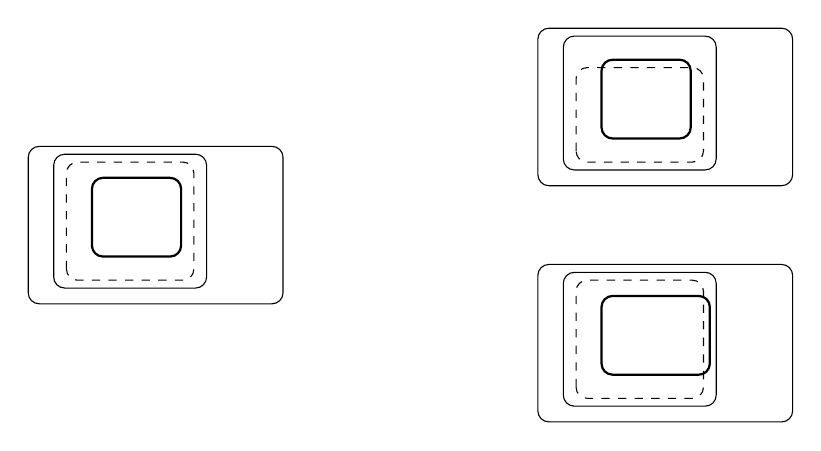
\begin{tikzpicture}
    \pgfmathsetmacro\gr{1.61803}
    \pgfmathsetmacro\by{2}
    \pgfmathsetmacro\bx{\by*\gr}

    \pgfmathsetmacro\pw{\bx*2.5}
    \pgfmathsetmacro\ph{\by*2.5}

    % % % Initial model % % %
    \pgfmathsetmacro\initX{-(\bx)}
    \pgfmathsetmacro\initY{(\ph - \by)/2}

    \draw[rounded corners] (\initX,\initY) rectangle (\initX + \bx,\initY + \by);

    \draw[rounded corners] (\initX +\bx*0.1, \initY + \by*0.1) rectangle (\initX + \bx*0.7,\initY + \by*0.95); % P
    \draw[rounded corners, dashed] (\initX + \bx*0.15,\initY +\by*0.15) rectangle (\initX + \bx*0.65,\initY + \by*0.9);

    \draw[rounded corners, thick] (\initX + \bx*0.25,\initY + \by*0.3) rectangle (\initX + \bx*0.6,\initY + \by*0.8); % Desire

    % % % Slip One % % %
    \pgfmathsetmacro\slipOneX{\bx}
    \pgfmathsetmacro\slipOneY{(\ph - \by)}

    \draw[rounded corners] (\slipOneX,\slipOneY) rectangle (\slipOneX + \bx,\slipOneY + \by);

    \draw[rounded corners] (\slipOneX + \bx*0.1, \slipOneY + \by*0.1) rectangle (\slipOneX + \bx*0.7,\slipOneY + \by*0.95); % P
    \draw[rounded corners, dashed] (\slipOneX + \bx*0.15,\slipOneY + \by*0.15) rectangle (\slipOneX + \bx*0.65,\slipOneY + \by*0.75);

    \draw[rounded corners, thick] (\slipOneX + \bx*0.25, \slipOneY + \by*0.3) rectangle (\slipOneX + \bx*0.6, \slipOneY + \by*0.8); % Desire

    % % % Slip Two % % %
    \pgfmathsetmacro\slipTwoX{\bx}
    \pgfmathsetmacro\slipTwoY{0}

    \draw[rounded corners] (\slipTwoX,\slipTwoY) rectangle (\slipTwoX + \bx,\slipTwoY + \by);

    \draw[rounded corners] (\slipTwoX + \bx*0.1,\slipTwoY + \by*0.1) rectangle (\slipTwoX + \bx*0.7,\slipTwoY + \by*0.95); % P
    \draw[rounded corners, dashed] (\slipTwoX + \bx*0.15,\slipTwoY +\by*0.15) rectangle (\slipTwoX + \bx*0.65,\slipTwoY + \by*0.9);

    \draw[rounded corners, thick] (\slipTwoX + \bx*0.25,\slipTwoY + \by*0.3) rectangle (\slipTwoX + \bx*0.675,\slipTwoY + \by*0.8); % Desire
  \end{tikzpicture}
  \caption{Dynamic slips}
\end{figure}

Conservative with respect to an expression, in the sense that although certain expressions no longer hold relevant significance, the agent's application of the expression can recover the previous instance.
Here we have applicative and desiderative slips.
These terms aren't great, but they sort of work.

But there are also extreme cases of slips, such as when the expression completely slips from the agent's resources.

\begin{figure}[!ht]
  \centering
  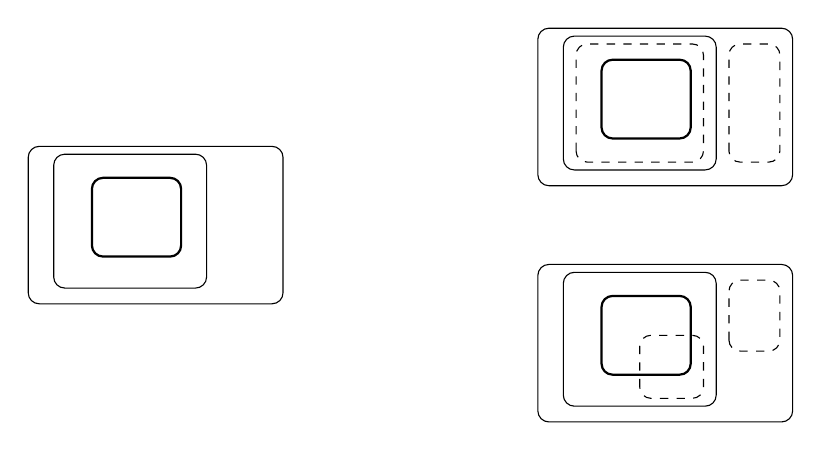
\begin{tikzpicture}
    \pgfmathsetmacro\gr{1.61803}
    \pgfmathsetmacro\by{2}
    \pgfmathsetmacro\bx{\by*\gr}

    \pgfmathsetmacro\pw{\bx*2.5}
    \pgfmathsetmacro\ph{\by*2.5}

    % % % Initial model % % %
    \pgfmathsetmacro\initX{-(\bx)}
    \pgfmathsetmacro\initY{(\ph - \by)/2}

    \draw[rounded corners] (\initX,\initY) rectangle (\initX + \bx,\initY + \by);

    \draw[rounded corners] (\initX +\bx*0.1, \initY + \by*0.1) rectangle (\initX + \bx*0.7,\initY + \by*0.95); % P
    % \draw[rounded corners, dashed] (\initX + \bx*0.15,\initY +\by*0.15) rectangle (\initX + \bx*0.65,\initY + \by*0.9);

    \draw[rounded corners, thick] (\initX + \bx*0.25,\initY + \by*0.3) rectangle (\initX + \bx*0.6,\initY + \by*0.8); % Desire

    % % % Might One % % %
    \pgfmathsetmacro\mightOneX{\bx}
    \pgfmathsetmacro\mightOneY{\ph - \by}

    \draw[rounded corners] (\mightOneX,\mightOneY) rectangle (\mightOneX + \bx,\mightOneY + \by);

    \draw[rounded corners] (\mightOneX + \bx*0.1, \mightOneY + \by*0.1) rectangle (\mightOneX + \bx*0.7,\mightOneY + \by*0.95); % P
    \draw[rounded corners, dashed] (\mightOneX + \bx*0.15,\mightOneY +\by*0.15) rectangle (\mightOneX + \bx*0.65,\mightOneY + \by*0.9);
     \draw[rounded corners, dashed] (\mightOneX + \bx*0.75,\mightOneY +\by*0.15) rectangle (\mightOneX + \bx*0.95,\mightOneY + \by*0.9);


    \draw[rounded corners, thick] (\mightOneX + \bx*0.25, \mightOneY + \by*0.3) rectangle (\mightOneX + \bx*0.6, \mightOneY + \by*0.8); % Desire

    % % % Might Two % % %
    \pgfmathsetmacro\mightTwoX{\bx}
    \pgfmathsetmacro\mightTwoY{0}

    \draw[rounded corners] (\mightTwoX,\mightTwoY) rectangle (\mightTwoX + \bx,\mightTwoY + \by);

    \draw[rounded corners] (\mightTwoX + \bx*0.1,\mightTwoY + \by*0.1) rectangle (\mightTwoX + \bx*0.7,\mightTwoY + \by*0.95); % P
    \draw[rounded corners, dashed] (\mightTwoX + \bx*0.4,\mightTwoY +\by*0.15) rectangle (\mightTwoX + \bx*0.65,\mightTwoY + \by*0.55);
    \draw[rounded corners, dashed] (\mightTwoX + \bx*0.75,\mightTwoY +\by*0.45) rectangle (\mightTwoX + \bx*0.95,\mightTwoY + \by*0.9);

    \draw[rounded corners, thick] (\mightTwoX + \bx*0.25, \mightTwoY + \by*0.3) rectangle (\mightTwoX + \bx*0.6, \mightTwoY + \by*0.8); % Desire
  \end{tikzpicture}
  \caption{Dynamic might}
\end{figure}

Here we suppose that the agent doesn't do anything with some expression.
Two uses of `might'.
First, to update the agent's application of an expression.
Second, to describe the result.
With the update, things can go well, when describing we typically have the bad case in mind.

Could also float the idea of a desiderative might.
So, forming the means for something which may of may not satisfy the agent.
This is the ice cream style example.
Certain abuse of the model is required here.
As need to pick some arbitrary collection of situations, something that the agent doesn't have the resources to evaluate.
But I think this is fine, because the guiding interpretation is that the attentive component is enough to evaluate.
That is, there are still the truth values hanging about, and hence the agent can do something with these, even if they don't know how to evaluate them.




These are the two key dynamics we need.
First there's a fixed `slip', then there's a successful might.
At least, this is all that's needed from a very general perspective.
What we haven't captured is the way that the means help recover the end.

Here is where belief becomes important.
Basically, belief picks out a subset of situations, using the fact that you want to hear the song again.
Then, you lose the information and your belief expands.
You then rule out certain situations.
And eventually there's a might again.





\begin{figure}[ht]
  \centering
  \begin{subfigure}[b]{0.3\textwidth}
    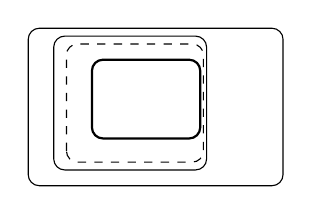
\begin{tikzpicture}
      \pgfmathsetmacro\gr{1.61803}
      \pgfmathsetmacro\by{2}
      \pgfmathsetmacro\bx{\by*\gr}
      \draw[rounded corners] (0,0) rectangle (\bx,\by);

      \draw[rounded corners] (\bx*0.1, \by*0.1) rectangle (\bx*0.7,\by*0.95); % P

      \draw[rounded corners, dashed] (\bx*0.15,\by*0.15) rectangle (\bx*0.6875,\by*0.9);

      \draw[rounded corners, thick] (\bx*0.25, \by*0.3) rectangle (\bx*0.675,\by*0.8); % Desire
    \end{tikzpicture}
    \caption{Both}
  \end{subfigure}
\end{figure}




\begin{figure}[ht]
  \centering
  \begin{subfigure}[b]{0.3\textwidth}
    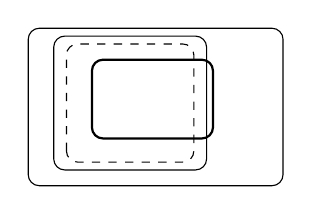
\begin{tikzpicture}
      \pgfmathsetmacro\gr{1.61803}
      \pgfmathsetmacro\by{2}
      \pgfmathsetmacro\bx{\by*\gr}
      \draw[rounded corners] (0,0) rectangle (\bx,\by);

      \draw[rounded corners] (\bx*0.1, \by*0.1) rectangle (\bx*0.7,\by*0.95); % P

      \draw[rounded corners, dashed] (\bx*0.15,\by*0.15) rectangle (\bx*0.65,\by*0.9);

      \draw[rounded corners, thick] (\bx*0.25, \by*0.3) rectangle (\bx*0.725,\by*0.8); % Desire
    \end{tikzpicture}
    \caption{Difficult}
  \end{subfigure}
  \caption{Three different `updates'}
\end{figure}



\newpage


\section{Logic Notes}
\label{sec:logic-notes}

\begin{proposition}
  The up and down versions of mental operators are not interdefinable.
  \begin{proof}
    Consider \(\ldesd{p} \rightarrow \lnot p\).

    Suppose a frame is not irreflexive. Then, value the relflexive point \(p\), and the formula is false at this point.

    Conversely, suppose the formula is invalid.
    Then \(\ldesd{p} \land p\) for some point, which means that this point must be accessible from itself, and hence the frame cannot be irreflexive.
  \end{proof}
\end{proposition}


\begin{example}
  The two sub-consequence relations are distinct.
  For example: \(p \lint q \vDash \ast, q\), but \(p \lint q \nvDash q\).
  {\color{red} It's not clear that this kind of thing holds for classical logical operators.}
\end{example}



\subsection{Sequential Rules}
\label{sec:sequential-rules}

\subsubsection{Structural Rules}
\label{sec:structural-rules}

four structural rules, more or less standard.

\begin{prooftree}
  \def\fCenter{\mbox{\ \(\cap\)\ }}
  \Axiom\(\Gamma \fCenter\ \Delta \ne \emptyset\)
  \RightLabel{\ruleStart}
  \deffCenter
  \UnaryInf\(\Gamma \fCenter\ \Delta\)
\end{prooftree}



\begin{multicols}{2}
  \begin{prooftree}
    \Axiom\(\Gamma \fCenter\ \Delta\)
    \def\fCenter{\mbox{\ \(\subseteq\)\ }}
    \Axiom\(\Delta \fCenter\ \Delta'\)
    \RightLabel{\ruleMonR}
    \deffCenter
    \BinaryInf\(\Gamma \fCenter\ \Delta'\)
  \end{prooftree}

\begin{prooftree}
  \Axiom\(\Gamma \fCenter\ \Delta\)
  \def\fCenter{\mbox{\ \(\subseteq\)\ }}
  \Axiom\(\Gamma \fCenter\ \Gamma'\)
  \RightLabel{\ruleMonL}
  \deffCenter
  \BinaryInf\(\Gamma' \fCenter\ \Delta\)
\end{prooftree}
\end{multicols}

\begin{prooftree}
  \Axiom\(\Gamma, \phi \fCenter \Delta\)
  \Axiom\(\Gamma \fCenter \phi, \Delta\)\RightLabel{\ruleCut}
  \BinaryInf\(\Gamma \fCenter \Delta\)
\end{prooftree}

\subsubsection{Propositional rules}
\label{sec:propositional-rules}

Collection of general propositional rules which are valid for any type of formula.

\begin{multicols}{2}
  \begin{prooftree}
    \AxiomEmpty
    \RightLabel{\ruleTop}
    \UnaryInf\(\fCenter \top\)
  \end{prooftree}

  \begin{prooftree}
    \AxiomEmpty
    \RightLabel{\ruleBot}
    \UnaryInf\(\bot \fCenter\)
  \end{prooftree}
\end{multicols}

\begin{multicols}{2}
  \begin{prooftree}
    \AxiomEmpty
    \RightLabel{\ruleNotAstL}
    \UnaryInf\(\lnot\ast \fCenter \ast\)
  \end{prooftree}

  \begin{prooftree}
    \AxiomEmpty
    \RightLabel{\ruleNotAstR}
    \UnaryInf\(\ast \fCenter \lnot\ast\)
  \end{prooftree}
\end{multicols}

\begin{multicols}{2}
  \begin{prooftree}
    \AxiomEmpty
    \RightLabel{\ruleAstL}
    \UnaryInf\(\phi,\lnot\phi \fCenter \ast\)
  \end{prooftree}

  \begin{prooftree}
    \AxiomEmpty
    \RightLabel{\ruleAstR}
    \UnaryInf\(\ast \fCenter \phi,\lnot\phi\)
  \end{prooftree}
\end{multicols}


\begin{multicols}{2}
  \begin{prooftree}
    \Axiom\(\lnot\Gamma \fCenter \Delta\)
    \RightLabel{\ruleNotL}
  \UnaryInf\(\lnot\Delta \fCenter \Gamma\)
\end{prooftree}
\columnbreak

\begin{prooftree}
  \Axiom\(\Gamma \fCenter\ \lnot\Delta\)
  \RightLabel{\ruleNotR}
  \UnaryInf\(\Delta \fCenter\ \lnot\Gamma\)
\end{prooftree}
\end{multicols}

\begin{multicols}{2}
  \begin{prooftree}
    \Axiom\(\Gamma,\phi,\psi \fCenter\ \Delta\)
    \doubleLine
    \RightLabel{\ruleAndL}
    \UnaryInf\(\Gamma,\phi\land\psi \fCenter\ \Delta\)
  \end{prooftree}

  \begin{prooftree}
    \Axiom\(\Gamma \fCenter\ \phi,\psi, \Delta\)
    \RightLabel{\ruleOrR}
    \doubleLine
    \UnaryInf\(\Gamma \fCenter\ \phi\lor\psi, \Delta\)
  \end{prooftree}
\end{multicols}


\begin{multicols}{2}
  \begin{prooftree}
    \Axiom\(\Gamma,\phi,\psi \fCenter\ \ast, \Delta\)
    \doubleLine
    \RightLabel{\ruleIntL}
    \UnaryInf\(\Gamma,\phi\lint\psi \fCenter\ \ast, \Delta\)
  \end{prooftree}

  \begin{prooftree}
    \Axiom\(\Gamma,\ast \fCenter\ \phi,\psi, \Delta\)
    \RightLabel{\ruleIntR}
    \doubleLine
    \UnaryInf\(\Gamma,\ast \fCenter\ \phi\lint\psi, \Delta\)
  \end{prooftree}
\end{multicols}

These are supplemented with two collections of special rules.
One for partial propositions and the other for total propositions.

For partial propositions we ensure consistency with a pair of fairly heavy-handed rules.
Note these are not hold in both directions.

\begin{multicols}{2}
  \begin{prooftree}
    \Axiom\(\Gamma,\attn{\phi} \fCenter\ \Delta\)
    \RightLabel{\ruleAttnL}
    \UnaryInf\(\Gamma,\attn{\phi},\phi \fCenter\ \Delta\)
  \end{prooftree}

  \begin{prooftree}
    \Axiom\(\Gamma \fCenter\ \attn{\phi}, \Delta\)
    \RightLabel{\ruleAttnR}
    \UnaryInf\(\Gamma \fCenter\ \attn{\phi} \land \phi, \Delta\)
  \end{prooftree}
\end{multicols}

Finally, we ensure that `classical' propositions are bivalent.

\begin{prooftree}
    \AxiomC{\(\attn{\psi} \notin \text{\emph{Sub}}(\phi)\)}
    \RightLabel{\ruleClassical}
    \UnaryInfC{\(\fCenter\ \phi,\lnot\phi\)}
  \end{prooftree}


\subsubsection{Modal Rules}
\label{sec:modal-rules}

Following \citeauthor{Jaspars:1996aa}, we introduce a single rule covering the general semantics of \(\Box\)-type formulas in our system.
This rule is termed general as it does not depend on the constraints we place on accessibility relations.

\begin{prooftree}
  \Axiom\(\Gamma \fCenter\ \phi, \lnot\Delta\)
  \RightLabel{\ruleBoxR}
  \UnaryInf\(\Box\Gamma \fCenter\ \Box\phi, \lnot\Box\Delta\)
\end{prooftree}

\begin{lemma}[Soundness]
  Rule \ruleBoxR\ is sound.
  \begin{proof}
    Suppose \(\Gamma \Vdash \phi, \lnot\Delta\).

    For the left-to-right direction suppose for some \(s \in \omodel{M}\), \(\omodel{M},s \vDash \Box\gamma\) for all \(\gamma \in \Gamma\) and let \(t\) be arbitrary such that \(Rst\).
    From the above, \(\omodel{M},t \vDash \gamma\) for all \(\gamma \in \Gamma\) and therefore \(\omodel{M},t \vDash \phi\) or \(\omodel{M},t \vDash \lnot\delta\) for some \(\delta \in \Delta\).
    If it is the case that \(\omodel{M},v \vDash \phi\) for every \(v\) such that \(Rsv\) then clearly \(\omodel{M},s \vDash \Box\phi\), while if there is some \(v\) such that \(Rsv\) while \(\omodel{M},v \nvDash \phi\) then \(\omodel{M},v \vDash \lnot\delta\) for some \(\delta \in \Delta\) and hence \(\omodel{M},s \vDash \lnot\Box\delta\).

    For the right-to-left direction suppose for some \(s \in \omodel{M}\), \(\omodel{M},s \Dashv \Box\phi\) and \(\omodel{M},s \Dashv \lnot\Box\delta\) for every \(\delta \in \Delta\).
    So, \(\omodel{M},s \vDash \lnot\Box\phi\) and \(\omodel{M},s \vDash \Box\delta\) for every \(\delta \in \Delta\).
    By the former conjunct there is some \(t \in \omodel{M}\) such that \(Rst\) with \(\omodel{M},t \vDash \lnot\phi\) and by the latter conjunct \(\omodel{M},t \vDash \delta\) for every \(\delta \in \Delta\).
    Our assumption that \(\Gamma \Vdash \phi, \lnot\Delta\) ensure that \(\Delta, \lnot\phi \Vdash \lnot\Gamma\) and hence it must be the case that \(\omodel{M},t \vDash \lnot\gamma\) for some \(\gamma \in \Gamma\) and hence \(\omodel{M},s \Dashv \Box\gamma\) for some \(\gamma \in \Gamma\).
  \end{proof}
\end{lemma}

\begin{proposition}
  The following rules are derivable:
  \begin{multicols}{2}
    \begin{prooftree}
      \Axiom\(\Gamma,\lnot\phi \fCenter\ \lnot\Delta\)
      \RightLabel{\ruleBoxLP}
      \UnaryInf\(\Box\Gamma,\lnot\Box\phi \fCenter\ \lnot\Box\Delta\)
    \end{prooftree}

  \begin{prooftree}
    \Axiom\(\Gamma,\phi \fCenter\ \Delta\)
    \RightLabel{\ruleDiaL}
    \UnaryInf\(\Box\Gamma,\Diamond\phi \fCenter\ \Diamond\Delta\)
  \end{prooftree}
\end{multicols}

  \begin{proof}
    By applying the contraposition rule.
  \end{proof}
\end{proposition}
\citeauthor{Jaspars:1996aa} require \ruleBoxLP\ to be taken as a separate rule due to the consequence relation they use.

Window-type modalities are governed by a corresponding rule.

\begin{prooftree}
  \Axiom\(\lnot\Gamma \fCenter\ \phi, \Delta\)
  \RightLabel{\ruleWinR}
  \UnaryInf\(\Window\Gamma \fCenter\ \Window\lnot\phi, \lnot\Window\Delta\)
\end{prooftree}

\ruleWinR\ is structurally similar to \ruleBoxR, but `flipped' to account for the relation to
inaccessible states.


\begin{proposition}
  Rule \ruleWinR\ is sound.
  \begin{proof}
    Assume \(\lnot\Gamma \Vdash \phi, \Delta\).

    For the left-to-right direction suppose for some \(s \in \omodel{M}\), \(\omodel{M},s \vDash \Window\gamma\) for all \(\gamma \in \Gamma\).
    By the semantic clause for \(\Window\) we have for all \(t\) such that \(\lnot Rst\), \(\omodel{M}, t \vDash \lnot\gamma\) for all \(\gamma \in \Gamma\).
    If it is the case that \(\omodel{M},v \vDash \phi\) for every \(v\) such that \(\lnot Rsv\) then clearly \(\omodel{M},s \vDash \Window\lnot\phi\).
    And, if there is some \(v\) such that \(\omodel{M},v \nvDash \phi\), then \(\omodel{M},v \vDash \delta\) for some \(\delta \in \Delta\) from which it follows that \(\omodel{M},s \vDash \lnot\Window\delta\).

    For the right-to-left direction, suppose \(\omodel{M}, s \Dashv \Window\lnot\phi\) and \(\omodel{M},s \Dashv \lnot\Window\delta\) for all \(\delta \in \Delta\).
    Hence, \(\omodel{M},s \vDash \Kite\phi\) and \(\omodel{M},s \vDash \Window\delta\) for \(\delta \in \Delta\).
    By the former there is some \(t \in \omodel{M}\) such that \(\lnot Rst\) with \(\omodel{M}, t \vDash \lnot\phi\) and by the latter it is also the case that \(\omodel{M},t \vDash \lnot\delta\) for each \(\delta \in \Delta\).
    As \(\lnot\Gamma \Vdash \phi, \lnot\Delta\) we also have \(\lnot\Delta \Vdash, \lnot\phi \Vdash \Gamma\), and hence \(\omodel{M},t \vDash \gamma\) for some \(\gamma \in \Gamma\).
    Therefore, \(\omodel{M},s \Dashv \Window\gamma\) for some \(\gamma \in \Gamma\).
  \end{proof}
\end{proposition}

\begin{proposition}
  The following rules are derivable:
  \begin{multicols}{2}
    \begin{prooftree}
  \Axiom\(\lnot\Gamma,\lnot\phi \fCenter\ \lnot\Delta\)
  \RightLabel{\ruleWinL}
  \UnaryInf\(\Window\Gamma,\lnot\Window\phi \fCenter\ \lnot\Window\Delta\)
\end{prooftree}

\begin{prooftree}
  \Axiom\(\lnot\Gamma,\lnot\phi \fCenter\ \lnot\Delta\)
  \RightLabel{\ruleKitL}
  \UnaryInf\(\Window\Gamma,\Kite\phi \fCenter\ \Kite\Delta\)
\end{prooftree}
  \end{multicols}
\end{proposition}

The interaction between \(\Box\) and \(\Window\) is split into five additional axioms.
% Combined, these ensure the global modality \(\Global\) (where \(\Global\phi \coloneq \Box\phi \land \Window\lnot\phi\)) is an S5 modality and correspond to the standard modal axioms M, 4, and B, respectively.

\begin{prooftree}
  \AxiomEmpty
  \RightLabel{\ruleGlobalM}
  \UnaryInf\(\Box\phi, \Window\lnot\phi \fCenter\ \phi\)
\end{prooftree}

\begin{prooftree}
  \AxiomEmpty
  \RightLabel{\ruleGlobalF}
  \UnaryInf\(\Box\phi, \Window\lnot\phi \fCenter\ \Box(\Box\phi \land \Window\lnot\phi) \land \Window\lnot(\Box\phi \land \Window\lnot\phi)\)
\end{prooftree}

\begin{prooftree}
  \AxiomEmpty
  \RightLabel{\ruleGlobalB}
  \UnaryInf\(\phi \fCenter\ \Box\lnot(\Box\lnot\phi \land \Window\phi) \land \Window(\Box\lnot\phi \land \Window\phi)\)
\end{prooftree}

For the reflexivity of the joint relation, I have:
\begin{prooftree}
  \AxiomEmpty
  \UnaryInf\(\phi, \Window\lnot\psi \fCenter\ \psi \lor \Diamond\phi\)
\end{prooftree}

% Four rules to deal with the interaction between \(\Box\) and \(\Window\).
% Each of these rules relies on the non-derivability of some modal formula.
% Intuition here is any state must be either accessible or inaccessible.
% With \ruleGlobalM\ we ensure that if some formula is true at a state then its relevance to satisfaction is recognised, but \ruleGlobalM\ does not, at least straightforwardly, ensure this holds for arbitrary collections of formulas.


% \begin{multicols}{2}
%   \begin{prooftree}
%     \AxiomC{\(\Gamma \vdash \phi \quad \Gamma \nvdash \psi \quad \Delta \vdash \Window\lnot\psi \land \Some\phi\)}
%     \UnaryInfC{\(\Delta \vdash \Diamond\phi\)}
%   \end{prooftree}
%   \begin{prooftree}
%      \AxiomC{\(\Gamma \vdash \phi \quad  \Gamma \nvdash \psi \quad \Delta \vdash \Box\psi \land \langle \Some\phi\)}
%     \UnaryInfC{\(\Delta \vdash \Kite\lnot\phi\)}
%   \end{prooftree}
% \end{multicols}


% \begin{multicols}{2}
%   \begin{prooftree}
%     \AxiomC{\(\Gamma \vdash \phi \quad \Gamma \vdash \psi \quad \Delta \nvdash \Diamond\phi\)}
%     \UnaryInfC{\(\Delta \vdash \Kite\lnot\psi\)}
%   \end{prooftree}
%   \begin{prooftree}
%      \AxiomC{\(\Gamma \vdash \phi \quad \Gamma \vdash \psi \quad \Delta \nvdash \Kite\lnot\phi\)}
%     \UnaryInfC{\(\Delta \vdash \Diamond\psi\)}
%   \end{prooftree}
% \end{multicols}

% I think with these four rules I get \(\modcou{\Box}{\Gamma} \subseteq \Delta \subseteq \modcou{\Diamond}{\Gamma}\) or the same for window whenever I have the global stuff working out.
% These are sound, and when I'm doing stuff with saturation, I may have a number of additional things, but I don't think this is going to be too much of a problem.
% Of course, I don't get anything like decidability.
% It's then interesting that these rules don't need to apply when \(\Delta = \Gamma\), but this doesn't give a clear way to eliminate for the general case.
% And, all of these rules are left-to-right only, I think.

% Wait, the last two rules \emph{can} be replaced.

% \begin{multicols}{2}
%   \begin{prooftree}
%     \AxiomC{\(\Gamma \vdash \phi \quad \Gamma \vdash \psi\)}
%     \UnaryInfC{\(\Delta \vdash \Diamond\phi \lor \Kite\lnot\psi\)}
%   \end{prooftree}
%   \begin{prooftree}
%      \AxiomC{\(\Gamma \vdash \phi \quad \Gamma \vdash \psi\)}
%     \UnaryInfC{\(\Delta \vdash \Diamond\psi \lor \Kite\lnot\phi\)}
%   \end{prooftree}
% \end{multicols}
% And these are, in fact, the same rule.
% And, these don't cover the reflexive case.
% And, they're a little different to rule \ruleGlobalM, I think.
% The trouble is, these two rules don't do any work, and it's only the top two rules that I actually need.


\subsection{Some useful properties}
\label{sec:some-usef-deriv}

\begin{proposition}[Finiteness]\label{prop:finiteness}
  \(\Gamma \vdash \Delta\) if and only if there exist finite \(\Gamma' \subseteq \Gamma\) and \(\Delta' \subseteq \Delta\) such that \(\Gamma' \vdash \Delta'\).
  \begin{proof}
    The left-to-right direction is by induction on the length of proofs.
    Base cases show how to find the finite sets, and then the rules only manipulate finite subsets.

    The right-to-left direction follows by monotonicity.
  \end{proof}
\end{proposition}

Terming finiteness `useful' may be an understatement, for without this property our method of proving completeness would fail.
However, we introduce the property here as it allows us to derive a pair of useful rules in proposition~\ref{prop:ContapositionRules} which we build up to.

\begin{proposition}\label{prop:DN}
  The following rules are derivable:
  \begin{multicols}{2}
    \begin{prooftree}
      \AxiomEmpty
      \UnaryInf\(\phi \fCenter\ \lnot\lnot\phi\)
    \end{prooftree}

    \begin{prooftree}
      \AxiomEmpty
      \UnaryInf\(\lnot\lnot\phi \fCenter\ \phi\)
    \end{prooftree}
  \end{multicols}
  \begin{proof}
    From \ruleStart\ we can obtain \(\lnot\phi \vdash \lnot\phi\).
    The left rule then follows by a single application of \ruleNotR\ and the right rule likewise follows from a single application of \ruleNotL.
  \end{proof}
\end{proposition}

\begin{proposition}\label{prop:DNSubst}
  The following rules are derivable:
  \begin{multicols}{2}
    \begin{prooftree}
      \Axiom\(\Gamma, \phi \fCenter\ \Delta\)
      \doubleLine
      \UnaryInf\(\Gamma, \lnot\lnot\phi \fCenter\ \Delta\)
    \end{prooftree}

    \begin{prooftree}
      \Axiom\(\Gamma \fCenter\ \phi, \Delta\)
      \doubleLine
      \UnaryInf\(\Gamma \fCenter\ \lnot\lnot\phi, \Delta\)
    \end{prooftree}
  \end{multicols}
  \begin{proof}
    We provide proofs of the downward instances of the rules, with the upward instances being analogous, viz:
    \begin{multicols}{2}
      \begin{prooftree}
        \Axiom\(\Gamma, \phi \fCenter\ \Delta\)
        \AxiomEmpty
        \UnaryInf\(\lnot\lnot\phi \fCenter\ \phi\)
        \UnaryInf\(\Gamma, \lnot\lnot\phi \fCenter\ \phi, \Delta\)
        \BinaryInf\(\Gamma, \lnot\lnot\phi \fCenter\ \Delta\)
      \end{prooftree}

      \begin{prooftree}
        \Axiom\(\Gamma \fCenter\ \phi, \Delta\)
        \AxiomEmpty
        \UnaryInf\(\phi \fCenter\ \lnot\lnot\phi\)
        \UnaryInf\(\Gamma, \phi \fCenter\ \lnot\lnot\phi, \Delta\)
        \BinaryInf\(\Gamma \fCenter\ \lnot\lnot\phi, \Delta\)
      \end{prooftree}
    \end{multicols}
  \end{proof}
\end{proposition}

\begin{proposition}\label{prop:ContapositionRules}
  The following rules are derivable:
  \begin{multicols}{2}
    \begin{prooftree}
      \Axiom\(\Gamma \fCenter\ \Delta\)
      \doubleLine
      \UnaryInf\(\lnot\Delta \fCenter\ \lnot\Gamma\)
    \end{prooftree}

    \begin{prooftree}
      \Axiom\(\Gamma \fCenter\ \lnot\Delta\)
      \doubleLine
      \UnaryInf\(\Delta \fCenter\ \lnot\Gamma\)
    \end{prooftree}
  \end{multicols}
  \begin{proof}
    If \(\Gamma \vdash (\lnot)\Delta\) then by proposition~\ref{prop:finiteness} there exist finite \(\Gamma' \subseteq \Gamma\) and \(\Delta' \subseteq (\lnot)\Delta\) such that \(\Gamma' \vdash \Delta'\).
    We can then apply the derived rules from proposition~\ref{prop:DNSubst} in conjunction with \ruleNotL\ and \ruleNotR\ to obtain the desire entailment between \(\Gamma'\) and \(\Delta'\) before appealing to \ruleMonL\ and \ruleMonR\ to obtain any `missing' formulas.
  \end{proof}
\end{proposition}

\begin{proposition}\label{prop:AstRules}
    The following rules are derivable:
   \begin{multicols}{2}
    \begin{prooftree}
      \Axiom\(\Gamma, \ast \fCenter\ \Delta\)
      \doubleLine
      \UnaryInf\(\Gamma, \lnot\ast \fCenter\ \Delta\)
    \end{prooftree}

    \begin{prooftree}
      \Axiom\(\Gamma \fCenter\ \ast, \Delta\)
      \doubleLine
      \UnaryInf\(\Gamma \fCenter\ \lnot\ast, \Delta\)
    \end{prooftree}
  \end{multicols}
  \begin{proof}
    Through rules \ruleNotAstL, \ruleNotAstR, \ruleMonL, \ruleMonL, and \ruleCut.
  \end{proof}
\end{proposition}


\subsection{Completeness Ideas}
\label{sec:completeness-ideas}

Completeness follows the traditional path of showing how to construct a countermodel for any failure of derivability.
The structural rule \ruleCut\ is important here.
For, if \(\Gamma \nvdash \Delta\), then \ruleCut\ guarantees there is no \(\lambda\) such that \(\Gamma,\lambda \vdash \Delta\) and \(\Gamma \vdash \lambda,\Delta\).
Spelt out, this means that there's no expression \(\lambda\) which connects \(\Gamma\) and \(\Delta\) by requiring that when every expression in \(\Gamma\) is true then some expression in \(\Delta\) must also be true and if every expression in \(\Delta\) is false then some expression in \(\Gamma\) is false.
Hence, it will be possible to expand \(\Gamma\) and \(\Delta\) to an exhaustive pair \(\Gamma'\) and \(\Delta'\) partitioning the language, which in turn will provide the basis for specifying a countermodel.



The exhaustive pair specifies a point.

\begin{note}
  The basic idea is to take pairs of formulas. The pairs of interest are those in which the consequence relation does not trivially hold. Due to there being two directions to consider, this requires keeping track of which direction is of interest. If these pairs were finite, we could potentially focus on one direction, but as these may be infinite, we can't appeal to the rule of contraposition in the proof system.

  The goal is to take any consistent pair, and show that it can be made exhaustive. These exhaustive pairs will then form the basis for the canonical model.

  Conjecture: Only one of the pairs is required, as any given pair can be flipped through negation. However, it's not clear that this can easily be proven prior to the truth lemma, which is what's grounding the intuition.
\end{note}






This allows us to split the consequence relation.
The use of this is to observe that there only needs to be one sub-failure of entailment.
This is, in part, what motivates the idea of taking exhaustive pairs.
For if \(\Gamma \nvdash \Delta\) then it must be the case that adding \(\ast\) to one of the sides preserves the failure.
Hence, we can potentially weaken while preserving the failure.
And, we don't need to directly deal with both sub-instances of entailment.





\begin{definition}[Consistency]
  Consistency is a mix of two conditions, because of the double-barrelled consequence relation.
  And, \(\ast\) is used this separates the two conditions.
  If a contradiction were used, this would lead to a stronger condition.
  \begin{itemize}
  \item \(\Gamma\) is consistent iff \(\Gamma \nvdash \ast\) or \(\ast \nvdash \Gamma\).
    \begin{itemize}
    \item Left consistency and right consistency, respectively.
    \end{itemize}
  \end{itemize}
  It turns out that either or the two conditions for consistency can be used, as a valuation for one condition can be inverted to provide a valuation for the other.
\end{definition}

Consistent sets will be saturated, and correspond to states.

The idea of saturation is key, but the double-barrelled notion of consequence requires some generalisations, as we may need to saturate for either truth or falsity.
\textcite{Thomason:1968aa} and \textcite{Aczel:1968aa} provide the foundations for saturated theories.

\begin{definition}[Saturation]
  Given a set of formulas \(\Gamma\), we say that \(\Gamma\) is:
  \begin{itemize}
  \item Left-saturated if for all \(\Sigma\), if \(\Gamma \vdash \ast, \Sigma\) then \(\Gamma \cap \Sigma \ne \emptyset\).
  \item Right-saturated if for all \(\Sigma\), if \(\Sigma, \ast \vdash \Gamma\) then \(\Gamma \cap \Sigma \ne \emptyset\).
  \end{itemize}
\end{definition}

\begin{definition}[Saturators]
  \mbox{ }
  \begin{itemize}
  \item \(\Lambda\) is a left saturator of \(\Gamma\) iff for all \(\Sigma\) if \(\Gamma \vdash \ast, \Sigma\) then \(\Sigma \cap \Lambda \ne \emptyset\)
  \item \(\Lambda\) is a right saturator of \(\Gamma\) iff for all \(\Sigma\) if \(\Sigma, \ast \vdash \Gamma\) then \(\Sigma \cap \Lambda \ne \emptyset\)
  \end{itemize}
\end{definition}


The Lindenbaum lemma is more involved than usual.
A saturated pair is either left or right saturated.
However, it may be possible for a pair to be either left or right saturated.
For example, \(\{p\}\).
Here, there are two exhaustive pairs, both of which would be fit for purpose.
Instead of choosing, we introduce two cases of saturation.

For left saturation, we immediately introduce an \(\ast\) on the right.
This weakens the consequence relation, as desired.

\begin{lemma}[Lindenbaum, left]\label{lindenbaum:left}
  Suppose \(\Lambda\) is a left saturator of \(\Gamma\), then there's a left-saturated set \(\Gamma^{+}\) such that \(\Gamma \subseteq \Gamma^{+} \subseteq \Lambda\).
  \begin{proof}
    Let \(\{\phi\}_{i_{i \in \omega}}\) be an enumeration of \(\olang{}\) such that every element of \(\Lambda\) occurs infinitely many times.\nolinebreak

    Given \(\{\phi\}_{i \in \omega}\), we define a sequence \(\{\Gamma_{i}\}_{i \in \omega}\) such that \(\Lambda\) is a left-saturator of each \(\Gamma_{i}\), with the limit of the sequence providing the desired left-saturated pair \(\Gamma^{+}\).

    \begin{align*}
      \Gamma_{0} &= \Gamma \\
      \Gamma_{n+1} &=
                                                  \begin{cases}
                                                    \Gamma_{n} \cup \{\phi_{n}\} &\text{if for all finite } \Sigma \colon \Sigma \cap \Lambda \ne \emptyset, \text{ when } \Gamma_{n},\phi_{n} \vdash \ast, \Sigma \\
                                                    \Gamma_{n}
                                                    &\text{otherwise} \\
                                                  \end{cases}
      \\
      \Gamma^{+} &= \bigcup_{n \in \omega}\Gamma_{n}
    \end{align*}

    To see that \(\Gamma^{+} \subseteq \Lambda\) note that by definition:
    \begin{enumerate}[label=(\arabic*)]
    \item\label{leftLindenbaum:1} if \(\Gamma_{n} \vdash \ast, \Sigma\) then \(\Sigma \cap \Lambda \ne \emptyset\) for all finite \(\Sigma \subseteq \olang{}\).
    \end{enumerate}
    By proposition~\ref{prop:finiteness} this means that \(\Lambda\) is a saturator of each \(\Gamma_{n}\), and so by some other observation we have \(\Gamma^{+} \subseteq \Lambda\).

    To establish the left-saturation of \(\Gamma^{+}\) we show that:
    \begin{enumerate}[label=(\arabic*),resume]
    \item\label{leftLindenbaum:2} For all \(k \in \omega \colon\) if \(\Gamma_{k} \vdash \ast, \Sigma\) and \(\Sigma\) is finite, then \(\Sigma \cap \Gamma^{+} \ne \emptyset\).
    \end{enumerate}

    This is where the repeated instances of a proposition in the enumeration \(\{\phi_{i}\}_{i \in \omega}\) comes into play.
    For, suppose that for some \(k\) and finite \(\Sigma\) it is the case that \(\Gamma_{k} \vdash \ast, \Sigma\) but \(\Sigma \cap \Gamma^{+} = \emptyset\).
    By~\ref{leftLindenbaum:1} we know that \(\Sigma \cap \Lambda\) is non-empty, and as each formula occurs in \(\{\phi_{i}\}_{i \in \omega}\) infinitely many times let \(\{\phi_{k_{1}}, \dots, \phi_{k_{n}}\}\) be an enumeration of \(\Sigma \cap \Lambda\) such that \(k < k_{i}\) for all \(i\) and \(k_{i} < k_{j}\) for \(i < j\).
    Intuitively, the enumeration \(\{\phi_{k_{1}}, \dots, \phi_{k_{n}}\}\) identifies some instance of each \(\phi \in \Sigma \cap \Lambda\) which are yet to be considered at the \(k^{\text{th}}\) stage of the sequence.

    For each \(\phi_{k_{i}}\) it must be that \mbox{\(\Gamma, \phi_{k_{i}} \vdash \ast, \Sigma_{i}\)} for some finite \(\Sigma_{i}\) such that \(\Sigma_{i} \cap \Lambda = \emptyset\), by the construction of \(\Gamma^{+}\).

    Still, \mbox{\(\Gamma_{k} \vdash \ast, \Sigma\)}, and so in particular \mbox{\(\Gamma_{k} \vdash \ast, \phi_{k_{i}},\Sigma - \{\phi_{k_{i}}\}\)} for each \(\phi_{k_{i}}\).
    Consider \mbox{\(\Gamma_{k} \vdash \ast, \phi_{k_{1}},\Sigma - \{\phi_{k_{1}}\}\)} and note that \mbox{\(\Gamma_{k_{1}}, \phi_{k_{1}} \vdash \ast, \Sigma_{1}\)}.
    From the latter two observations and an instance of Cut we obtain \mbox{\(\Gamma_{k}, \Gamma_{k_{1}} \vdash \ast, \Sigma - \{\phi_{k_{1}}\}, \Sigma_{1}\)}.
    And, as \mbox{\(\Gamma_{k} \subseteq \Gamma_{k_{1}}\)}, we can infer that \mbox{\(\Gamma_{k_{1}} \vdash \ast, \Sigma - \{\phi_{k_{1}}\}, \Sigma_{1}\)}.

    The previous steps can be replicated for each \(\phi_{k_{i}}\), noting that \(\Gamma_{k_{i}} \subseteq \phi_{k_{i+1}}\), from which we obtain \mbox{\(\Gamma_{k_{n}} \vdash \ast, \Sigma - \{\phi_{k_{1}},\dots,\phi_{k_{n}}\}, \Sigma_{1},\dots,\Sigma_{n}\)}.
    As \(\Sigma\) is finite by assumption, and each \(\Sigma_{i}\) is also finite (of which there are a finitely many), this means the union of the sets of the right hand side of the consequence relation is finite.
    Yet, \((\Sigma - \{\phi_{k_{1}},\dots,\phi_{k_{n}}\} \cup \Sigma_{1} \cup \dots \cup \Sigma_{n}) \cap \Lambda = \emptyset\), contradicting~\ref{leftLindenbaum:1}, above.

    So, for any finite \(\Gamma_{k}\), if \(\Gamma_{k} \vdash \ast, \Sigma\) and \(\Sigma\) is finite, then \(\Sigma \cap \Gamma^{+} \ne \emptyset\).

    By proposition~\ref{prop:finiteness}, if \(\Gamma^{+} \vdash \ast, \Sigma\) then there are finite subsets \(\Gamma \subseteq \Gamma^{+}\) and \(\Sigma' \subseteq \Sigma\) such that \(\Gamma \vdash \ast, \Sigma\) and by construction of \(\Gamma^{+}\) there is some \(n \in \omega\) such that \(\Gamma_{n} \vdash \ast, \Sigma'\).
    From \label{leftLindenbaum:2} we know that \(\Sigma' \cap \Gamma^{+} \ne \emptyset\) and so \(\Sigma \cap \Gamma^{+} \ne \emptyset\).
    Therefore, \(\Gamma^{+}\) is left-saturated.
  \end{proof}

\end{lemma}

For right saturation, we move our attention to the right-to-left sub-consequence relation.

\begin{lemma}[Lindenbaum, right]\label{lindenbaum:right}
  Suppose \(\Lambda\) is a right saturator of \(\Gamma\), then there's a right-saturated pair \(\Gamma^{+}\) such that \(\Gamma \subseteq \Gamma^{+} \subseteq \Lambda\).
  \begin{proof}
    The proof strategy for right-saturation is analogous to left-saturation, altered only for the corresponding change in sub-consequence relation of interest.
    \begin{align*}
      \Gamma_{0} &= \Gamma \\
      \Gamma_{n+1} &=
                                                  \begin{cases}
                                                    \Gamma_{n} \cup \{\phi_{n}\} &\text{if for all finite } \Sigma \colon \Sigma \cap \Lambda \ne \emptyset, \text{ when } \Sigma,\ast \vdash \phi_{n},\Gamma_{n} \\
                                                    \Gamma_{n} &\text{otherwise} \\
                                                  \end{cases}
      \\
      \Gamma^{+} &= \bigcup_{n \in \omega}\Gamma_{n}
    \end{align*}
    Again, \(\Gamma^{+}\) is exhaustive by construction and the following two properties can be established:
    \begin{enumerate}[label=(\arabic*)]
    \item\label{rightLindenbaum:1} If \(\Sigma,\ast \vdash \Gamma_{n}\) then \(\Sigma \cap \Lambda \ne \emptyset\) for all finite \(\Sigma\).
    \item\label{rightLindenbaum:2} For all \(k \in \omega \colon\) if \(\Sigma, \ast \vdash \Gamma_{k}\) and \(\Sigma\) is finite, then \(\Sigma \cap \Gamma^{+} \ne \emptyset\).
    \end{enumerate}
  \end{proof}
\end{lemma}



\begin{corollary}[Saturation]
  If \(\Gamma \nvdash \Delta\) then there exists a saturated set \(\Gamma^{+}\) such that \(\Gamma^{+} \cap \Delta = \emptyset\) with \(\Gamma \subseteq \Gamma^{+}\) where either
  \begin{enumerate}
  \item \(\Gamma^{+}\) is left-saturated if \(\Gamma \nvdash \ast, \Delta\), or
  \item \(\Gamma^{+}\) is right-saturated if \(\Delta,\ast \nvdash \Gamma\)
  \end{enumerate}
  \begin{proof}
    If \(\Gamma \nvdash \Delta\) then either \(\Gamma \nvdash \ast, \Delta\) or \(\Gamma, \ast \nvdash \Delta\).

    Suppose \(\Gamma \nvdash \ast, \Delta\).
    Then, \(\Delta^{c} = \olang{} - \Delta\) is a left-saturator of \(\Gamma\).
    For, \(\Delta^{c}\) is \emph{not} a saturator of \(\Gamma\) if and only if there is some \(\Sigma\) such that \(\Gamma \vdash \ast, \Sigma\) with \(\Sigma \cap \Delta^{c} = \emptyset\).
    Yet, if \(\Sigma \cap \Delta^{c} = \emptyset\), then \(\Sigma \subseteq \Delta\), and so by \ruleMonR\ the previous is the case if and only if \(\Gamma \vdash \ast, \Delta\) contradicting our initial assumption.

    So, as \(\Delta^{c}\) is a left-saturator of \(\Gamma\) and appeal to lemma~\ref{lindenbaum:left} ensures there is a left-saturated pair \(\Gamma^{+}\) such that \(\Gamma \subseteq \Gamma^{+} \subseteq \Delta^{c}\) and hence \(\Gamma^{+} \cap \Delta = \emptyset\).

    Likewise, if \(\Delta, \ast \nvdash \Gamma\) then \(\Delta^{c}\) is a right-saturator of \(\Gamma\) we appeal to lemma~\ref{lindenbaum:right} to find a right-saturated pair \(\Gamma^{+}\) with the desired properties.
  \end{proof}
\end{corollary}

The following lemma shows that lemmas~\ref{lindenbaum:left} and~\ref{lindenbaum:right} amount to the same thing, and either can be indirectly used to prove the other.\nolinebreak
\footnote{This is a version of \citeauthor{Blamey:1980aa}'s lemma III.2.15 (\citeyear[122]{Blamey:1980aa})}

\begin{lemma}[Correspondence]\label{lem:correspondence}
  \(\Gamma\) is left-saturated iff \(\lnot\Gamma\) is right-saturated.
  \begin{proof}
    From left to right, if \(\Gamma\) is left-saturated then, for finite \(\Sigma\), whenever \(\Gamma \vdash \Sigma\), \(\Gamma \cap \Sigma \ne \emptyset\).
    Suppose for some finite \(\Sigma'\), \(\Sigma' \vdash \lnot\Gamma\).
    Then, \(\Gamma \vdash \lnot\Sigma'\), by proposition~\ref{prop:ContapositionRules}.
    However, by the above this means that \(\Gamma \cap \lnot\Sigma' \ne \emptyset\), from which it follows that \(\lnot\Gamma \cap \Sigma' \ne \emptyset\), as if \(\phi \in \Gamma \cap \lnot\Sigma'\) then \(\phi \in \Gamma\) and \(\phi \in \lnot\Sigma'\) which ensures that \(\lnot\phi \in \lnot\Gamma\) and \(\lnot\phi \in \Sigma'\).
  \end{proof}
\end{lemma}

The primary use of lemma~\ref{lem:correspondence} will be to simplify our canonical model.
For, instead of taking saturated pairs in general, we may take either left- or right-saturated pairs without loss of generality, reducing the number of cases we need to consider when establishing the relevant truth lemma.

\begin{proposition}
  If \(\Gamma\) is left-saturated then for all \(\phi,\psi \in \olang{}\):
  \begin{enumerate}
  \item If \(\Gamma \vdash \ast, \phi\) then \(\phi \in \Gamma\).
  \item If \(\Gamma \vdash \ast, \phi \lor \psi\) then \(\Gamma \vdash \ast, \phi\) or \(\Gamma \vdash \ast, \psi\).
  \end{enumerate}
  \begin{proof}
    Both are immediate by the definition of left saturation.
    For if \(\Gamma \vdash \ast, \phi\) and \(\Gamma\) is left-saturated, then \(\Gamma \cap \{\phi\} \ne \emptyset\), hence \(\phi \in \Gamma\).
    Likewise, if \(\Gamma \vdash \ast, \phi \lor \psi\) then \(\Gamma \vdash \ast, \phi, \psi\) and hence \(\Gamma \cap \{\phi,\psi\} \ne \emptyset\) and so \(\phi \in \Gamma\) or \(\psi \in \Gamma\) and hence by rules \ruleStart, \ruleMonL, and \ruleMonR, either \(\Gamma \vdash \ast,\phi\) or \(\Gamma \vdash \ast, \psi\).
  \end{proof}
\end{proposition}

\begin{note}
  if \(\Gamma\) is a left-saturated set, then for any formula \(\phi \in \olang{}\): \(\Gamma \vdash \ast, \phi\) iff \(\Gamma \vdash \phi\).
\end{note}

In the construction of left-saturated sets we focus on the left-to-right sub-consequence relation.
However, once the set is left-saturated, the right-to-left sub-consequence relation must also hold as there's a witness to any entailment that will be made false.


\subsection{The Caonical Model}
\label{sec:caonical-model}

\begin{definition}
  Let \(\Gamma\) be a left-saturated set, we introduce the following notation to capture certain modal counterparts of \(\Gamma\).
  \begin{multicols}{2}
    \begin{itemize}
    \item \(\modcou{\Box}{\Gamma} = \{\phi \mid \Box\phi \in \Gamma \}\)
    \item \(\modcou{\Diamond}{\Gamma} = \{\phi \mid \Diamond\phi \in \Gamma\}\)
    \end{itemize}
    \begin{itemize}
    \item \(\modcou{\Window}{\Gamma} = \{\lnot\phi \mid \Window\phi \in \Gamma\}\)
    \item \(\modcou{\Kite}{\Gamma} = \{\lnot\phi \mid \Kite\phi \in \Gamma\}\)
    \end{itemize}
  \end{multicols}
\end{definition}

The required interaction between Box- and Window-type modalities makes the direct construction of an \emph{oblique} canonical model difficult.
However, by adapting a technique developed by Dimiter Vakarelov and put to use by \citeauthor{Gargov:1987aa}, we can straightforwardly construct a non-oblique canonical model which is modally equivalent to an oblique model.

\begin{definition}[Canonical Model]
  \(\cmodel = (\cmodW,\cmodBox,\cmodWin,\cmodV)\) where:
  \begin{itemize}
  \item \(\cmodW\) is the set of all left-saturated sets.
  \item \(\Gamma \cmodBox \Delta\) iff \(\modcou{\Box}{\Gamma} \subseteq \Delta \subseteq \modcou{\Diamond}{\Gamma}\)
  \item \(\Gamma \cmodWin \Delta\) iff \(\modcou{\Window}{\Gamma} \subseteq \Delta \subseteq \modcou{\Kite}{\Gamma}\)
  \item \(\Gamma \in \cintp{p}\) iff \(p \in \Gamma\) and \(\Gamma \in \iintp{p}\) iff \(\lnot p \in \Gamma\).
  \end{itemize}
\end{definition}

The interpretation specified for the canonical model relies on the left-saturation of \(\Gamma\), for left-saturation is truth-truth.
If right-saturated sets were to be used, we would flip the definition to require \(\Gamma \in \cintp{p}\) iff \(\lnot p \in \Gamma\) and \(\Gamma \in \iintp{p}\) iff \(p \in \Gamma\).

This lemma is used to make the truth lemma quite straightforward.
The second pair of implications require some care, as we take the negation of any modal formula for the Winow-type modalities.
The definitions hide this, in order to make the quantification more straightforward.

\begin{lemma}
  For any \(\Gamma\), \(\Delta\) in \(\cmodW\).
  \begin{enumerate}[label=(\alph*)]
  \item\label{lemmma:ext:box} If \(\modcou{\Box}{\Gamma} \subseteq \Delta\) then there exists a \(\Delta' \subseteq \Delta\) such that \(\Gamma \cmodBox \Delta'\)
  \item\label{lemma:ext:dia} If \(\Delta \subseteq \modcou{\Diamond}{\Gamma}\) then there exists a \(\Delta \subseteq \Delta'\) such that \(\Gamma \cmodBox \Delta'\)
  \item\label{lemma:ext:win} If \(\modcou{\Window}{\Gamma} \subseteq \Delta\) then there exists a \(\Delta' \subseteq \Delta\) such that \(\Gamma \cmodWin \Delta'\)
  \item\label{lemma:ext:kit} If \(\Delta \subseteq \modcou{\Kite}{\Gamma}\) then there exists a \(\Delta \subseteq \Delta'\) such that \(\Gamma \cmodWin \Delta'\)
  \end{enumerate}
  \begin{proof}
    Take \(\Gamma,\Delta \in \cmodW\).
    \begin{description}
    \item[\ref{lemmma:ext:box}] Assume \(\modcou{\Box}{\Gamma} \subseteq \Delta\).
    Our goal is to show that:
    \begin{enumerate}
    \item For all finite \(\Sigma\): If \(\modcou{\Box}{\Gamma} \vdash \ast, \Sigma\) then \(\Sigma \cap \Delta \cap \modcou{\Diamond}{\Gamma} \ne \emptyset\)
    \end{enumerate}
    For, given this we know by proposition~\ref{prop:finiteness} that \(\Delta \cap \modcou{\Diamond}{\Gamma}\) is a left-saturator of \(\modcou{\Box}{\Gamma}\).
    Then, by lemma~\ref{lindenbaum:left} there must be some left-saturated \(\Delta^{'}\) such that \(\modcou{\Box}{\Gamma} \subseteq \Delta^{'} \subseteq \Delta \cap \modcou{\Diamond}{\Gamma}\).

    So, suppose \(\modcou{\Box}{\Gamma} \vdash \ast,\Sigma\) for some finite \(\Sigma\).
    As \(\modcou{\Box}{\Gamma} \subseteq \Delta\) and \(\Delta \in \cmodW\) we have \(\Sigma \cap \Delta \ne \emptyset\).
    Rewriting, we have \(\modcou{\Box}{\Gamma} \vdash \ast, \Sigma - \Delta,\Sigma \cap \Delta\), which can be rewritten again as \(\modcou{\Box}{\Gamma} \vdash \ast, \sigma, \Sigma \cap \Delta\), where \(\sigma \coloneq \bigvee(\Sigma - \Delta)\).
    By the application of derived rule \ruleBoxR\ we obtain \(\Gamma \vdash \ast, \Box\sigma, \Diamond(\Sigma \cap \Delta)\).
    As \(\Gamma\) is left-saturated, it must be the case that either \(\Box\sigma \in \Gamma\) or \(\Diamond(\Sigma \cap \Delta) \in \Gamma\).
    However, if \(\Box\sigma \in \Gamma\) then \(\sigma \in \modcou{\Box}{\Gamma}\) and so \(\sigma \in \Delta\).
    And, as \(\Delta\) is also left-saturated from the previous we would have \(\phi \in \Delta\) for some \(\phi \in \Sigma - \Delta\).
    This means \(\Diamond(\Sigma \cap \Delta) \in \Gamma\), which is equivalent to \(\Sigma \cap \Delta \cap \modcou{\Diamond}{\Gamma} \ne \emptyset\).

  \item[\ref{lemma:ext:dia}]
    Assume \(\Delta \subseteq \modcou{\Diamond}{\Gamma}\).
    Our goal is to show that \(\modcou{\Diamond}{\Gamma}\) is a left-saturator of \(\modcou{\Box}{\Gamma}\), for then by lemma~\ref{lindenbaum:left} there is some left-saturated set \(\Delta'\) such that \(\modcou{\Box}{\Gamma} \cup \Delta \subseteq \Delta' \subseteq \modcou{\Diamond}{\Gamma}\).
    The accessibility of \(\Delta'\) is then guaranteed by the simple fact that \(\modcou{\Box}{\Gamma} \subseteq \modcou{\Box}{\Gamma} \cup \Delta\).
    To do this we show:
    \begin{enumerate}[resume]
    \item For all finite \(\Sigma\): If \(\modcou{\Box}{\Gamma}, \Delta \vdash \ast, \Sigma\) then \(\Sigma \cap \modcou{\Diamond}{\Gamma} \ne \emptyset\).
    \end{enumerate}
    Suppose \(\modcou{\Box}{\Gamma}, \Delta \vdash \ast, \Sigma\).
    Then by proposition~\ref{prop:finiteness} then is some finite \(\Delta'\) such that \(\modcou{\Box}{\Gamma}, \Delta' \vdash \ast, \Sigma\).
    In turn, \(\modcou{\Box}{\Gamma}, \delta' \vdash \ast, \Sigma\), where \(\delta' \coloneq \bigwedge\Delta'\).
    So, by the derived rule \ruleDiaL\ we have \(\Gamma, \Diamond\delta' \vdash \ast, \Diamond\Sigma\).
    And, as \(\Delta\) is left-saturated we know \(\delta' \in \Delta\), and since \(\Delta \subseteq \modcou{\Diamond}{\Gamma}\) this means \(\Diamond\delta' \in \Gamma\).
    Combining the previous two observations, we see that \(\Gamma \vdash \ast, \Diamond\Sigma\), implying that \(\modcou{\Diamond}{\Gamma} \cap \Sigma \ne \emptyset\).
  \end{description}

  The second pair of implications follow the same strategy as the first pair.

  \begin{description}
  \item[\ref{lemma:ext:win}]
    Assume \(\modcou{\Window}{\Gamma} \subseteq \Delta\).
    As with the first implication, our goal is to show:
    \begin{enumerate}[resume]
    \item For all finite \(\Sigma\): If \(\modcou{\Window}{\Gamma} \vdash \ast, \Sigma\) then \(\Sigma \cap \Delta \cap \modcou{\Kite}{\Gamma} \ne \emptyset\).
    \end{enumerate}
    Suppose \(\modcou{\Window}{\Gamma} \vdash \ast, \Sigma\) for some finite \(\Sigma\).
    As \(\modcou{\Window}{\Gamma} \subseteq \Delta\) and \(\Delta \in \cmodW\) we have \(\Sigma \cap \Delta \ne \emptyset\), hence \(\modcou{\Window}{\Gamma} \vdash \ast, \Sigma - \Delta, \Sigma \cap \Delta\).
    Analogous to case~\ref{lemmma:ext:box}, rewriting and appealing to the derived rule \ruleKitL\ we obtain \(\modcou{\Window}{\Gamma} \vdash \ast, \Window\lnot\sigma, \Window(\Sigma \cap \Delta)\).
    So, if \(\Window\lnot\sigma \in \Gamma\) then \(\sigma \in \modcou{\Window}{\Gamma}\), which cannot be the case.
    Therefore, \(\Kite(\Sigma \cap \Delta) \in \Gamma\), which is equivalent to \(\Sigma \cap \Delta \cap \modcou{\Kite}{\Gamma} \ne \emptyset\).

  \item[\ref{lemma:ext:kit}]
    Assume \(\modcou{\Kite}{\Gamma} \subseteq \Delta\).
    As with the second implication, our goal is to show:
    \begin{enumerate}[resume]
    \item For all finite \(\Sigma\): If \(\modcou{\Window}{\Gamma}, \Delta \vdash \ast, \Sigma\) then \(\Sigma \cap \modcou{\Kite}{\Gamma} \ne \emptyset\).
    \end{enumerate}
    Analogous to the steps the second implication, suppose \(\modcou{\Window}{\Gamma}, \Delta \vdash \ast, \Sigma\) for some finite \(\Sigma\).
    Then by proposition~\ref{prop:finiteness} we have \(\modcou{\Window}{\Gamma}, \Delta' \vdash \ast, \Sigma\) for some finite \(\Delta' \subseteq \Delta\), and hence \(\modcou{\Window}{\Gamma}, \delta' \vdash \ast, \Sigma\) where \(\delta' \coloneq \bigwedge\Delta'\).
    By the derived rule \ruleKitL\ we obtain \(\Gamma, \Kite\lnot\delta' \vdash \ast, \Kite\Sigma\).
    As \(\Delta\) is left-saturated, \(\delta' \in \Delta\), and as \(\Delta \subseteq \modcou{\Kite}{\Gamma}\) this means \(\Kite\lnot\delta' \in \Gamma\).
    So, \(\modcou{\Window}{\Gamma} \vdash \ast, \Sigma\).
    \end{description}
  \end{proof}
\end{lemma}

\begin{lemma}
  For any \(\Gamma \in \cmodW\), either \(\modcou{\Box}{\Gamma} \subseteq \Gamma \subseteq  \modcou{\Diamond}{\Gamma}\) or \(\modcou{\Window}{\Gamma} \subseteq \Gamma \subseteq \modcou{\Kite}{\Gamma}\)
  \begin{proof}
    First we show that \(\modcou{\Box}{\Gamma} \subseteq \Gamma\) or \(\modcou{\Window}{\Gamma} \subseteq \Gamma\).
    For suppose not.
    Then there is some \(\Box\phi \in \Gamma\) such that \(\phi \notin \Gamma\) and some \(\Window\lnot\psi \in \Gamma\) such that \(\psi \notin \Gamma\).
    Hence, \(\Gamma \vdash \Box\phi\) and \(\Gamma \vdash \Window\lnot\psi\).

    As \(\phi \vdash \phi \lor \psi\), we know \(\Box\phi \vdash \Box(\phi \lor \psi)\) by \ruleBoxR\ and likewise as \(\lnot\lnot\psi \vdash \phi \lor \psi\) we obtain \(\Window\lnot\psi \vdash \Window\lnot(\phi \lor \psi)\) by \ruleWinR.
    Hence, \(\Gamma \vdash \Box(\phi \lor \psi) \land \Window\lnot(\phi \lor \psi)\).
    Therefore, by \ruleGlobalM\ we know \(\Gamma \vdash \phi \lor \psi\), but as \(\Gamma\) is left-saturated this means either \(\phi \in \Gamma\) or \(\psi \in \Gamma\) contradiction our initial assumption.

    Given \(\modcou{\Box}{\Gamma} \subseteq \Gamma\) or \(\modcou{\Window}{\Gamma} \subseteq \Gamma\) we now have two pairs of conditionals to prove:
    \begin{enumerate}
    \item
      \begin{enumerate*}
      \item If \(\modcou{\Window}{\Gamma} \nsubseteq \Gamma\) then \(\Gamma \subseteq \modcou{\Diamond}{\Gamma}\) \mbox{\quad }
      \item If \(\Gamma \nsubseteq \modcou{\Kite}{\Gamma}\) then \(\Gamma \subseteq \modcou{\Diamond}{\Gamma}\)
      \end{enumerate*}
    \item
      \begin{enumerate*}
      \item If \(\modcou{\Box}{\Gamma} \nsubseteq \Gamma\) then \(\Gamma \subseteq \modcou{\Kite}{\Gamma}\) \mbox{\quad }
      \item If \(\Gamma \nsubseteq \modcou{\Diamond}{\Gamma}\) then \(\Gamma \subseteq \modcou{\Kite}{\Gamma}\)
      \end{enumerate*}
    \end{enumerate}
    Suppose \(\modcou{\Window}{\Gamma} \nsubseteq \Gamma\).
    Then there is some \(\Window\lnot\psi \in \Gamma\) such that \(\psi \notin \Gamma\).
    Hence, as \(\Gamma \vdash \Window\lnot\psi\) and \(\Gamma \vdash \phi\) for any \(\phi \in \Gamma\) we know \(\Gamma \vdash \Window\lnot\psi \land \phi\).
    So, as we have both \(\Gamma \vdash \Window\lnot\psi \land \phi\) and \(\Gamma \nvdash \Window\lnot\psi\) we have \(\Gamma \vdash \Diamond\phi\) by rule {\color{red} the bottom left rule} which ensures that \(\Gamma \subseteq \modcou{\Diamond}{\Gamma}\).
  \end{proof}
\end{lemma}



We now establish the standard truth lemma for the canonical model.\nolinebreak
\footnote{If our model were to include right-saturated sets, we would require an additional truth lemma establishing that\(\Gamma \vDash \phi\) iff \(\lnot\phi \in \Gamma\) and \(\Gamma \Dashv \phi\) iff \(\phi \in \Gamma\).}

\begin{lemma}[Truth]
  For all \(\phi \in \olang{}\) and all left-saturated sets \(\Gamma\):
  \[\Gamma \vDash \phi\text{ iff }\phi \in \Gamma\text{ and }\Gamma \Dashv \phi\text{ iff }\lnot\phi \in \Gamma\]
  \begin{proof}

  \end{proof}
\end{lemma}

\newpage

\subsection{Still stuck on completeness}
\label{sec:still-stuck-compl}

If I know that \(\modcou{\Box}{\Gamma} \subseteq \Gamma\) or \(\modcou{\Window}{\Gamma}\) then I know that \(\modcou{\Diamond}{\Gamma} \subseteq \Gamma\) or \(\modcou{\Kite}{\Gamma}\) via the rules:
\[
  \phi,\Window\lnot\psi \vdash \psi \lor \Diamond\phi \quad \phi,\Box\psi \vdash \psi \lor \Kite\lnot\phi
\]
These are sound, because if \(\phi, \Window\lnot\psi\) are true at some state, then either the state is accessible and so \(\Diamond\phi\) holds, or the state is inaccessible and \(\psi\) holds.
Hence, when I know that one of the initial conditions obtains, I can get the other, at least with \(\Gamma\).

\[\Diamond\phi \land \Diamond\Window\lnot\psi \vdash \Diamond(\phi \land \psi), \Diamond(\Window\lnot\psi \land \Kite\lnot\phi)\]

From this I see that the \(\Window\lnot\psi\) state considers the \(\phi\) state either accessible or inaccessible, at least as far as the semantics goes.
That is, if the frame does not satisfy the condition then there's a counterexample to this.
For, take \(\phi\) to be an atom and suppose it only holds at a single state, and take some state with \(q\) holding at all inaccessible states.
Then if the window state doesn't consider the \(p\) state accessible, the latter disjunct won't hold, and if the \(p\) state isn't accessible then \(q\) won't hold with \(p\).

Same kind of frame idea and I can see
\[
  p \vdash \Box(\Diamond p \lor \Kite p)
\]
Must hold.

All of this is fine, but it only shows me that I am able to rule out a frame if I have arbitrary valuations are available to me.
This doesn't clearly establish anything about the canonical model, where I have a specific valuation.


\[
  \Diamond\Window\lnot\psi, \phi \vdash \ast, \psi, \Diamond\Diamond\phi
\]
As, the window world either considers the current world inaccessible and therefore \(\psi\) must hold, or the current world is accessible, and hence it's possible to go somewhere else and come back via the accessibility relation.
This doesn't force any accessible saturated set to include relevant diamond formulas, but it does mean that form the root world I can't rule out adding those diamond formulas to any saturated set which doesn't consider the root inaccessible.

The above can be strengthened to include additional depth.
\[
  \Diamond\Window\lnot\psi, \Diamond\Diamond\Window\lnot\psi, \phi \vdash \ast, \psi, \Diamond\Diamond\phi \land \Diamond\Diamond\Diamond\phi
\]
In fact, the number of diamonds prefixing the window modality correspond to the number of diamonds prefixing the formula true at the state plus one.

So, if I can build up some accessible state to ensure that the root is accessible from it, then I can likewise build up any other accessible state which accesses the pre-built-up state.

This also works for kite modalities.
Basically, it I can access a state which requires \(\psi\) at all inaccessible states, and \(\psi\) isn't true at the present state, then I can simply substitute the \(\Window\lnot\psi\) for a \(\Diamond\phi\).
\[
  \Diamond\Kite\lnot\Window\lnot\psi, \phi \vdash \ast, \psi, \Diamond\Kite\lnot\Diamond\phi \quad
  \Diamond\Diamond\Window\lnot\psi, \phi \vdash \ast, \psi, \Diamond\Diamond\Diamond\phi
\]
So, I get an infinite axiom schema of this form, whether I need this is unclear, but the initial cases sure seem useful.

The intuition here is that walking through the diamond modalities, I'm always one optional step away from returning to the current state, and that's all that's required.

So, if I have the potential to build up a saturated set, then I also see that any path I can take toward this set can be built up in a similar fashion.

The following axiom captures something of the connectedness requirement, and is a generalisation of the \(.3\) axiom of normal modal logic.
\[
  \Diamond\phi,
  \Some\psi
  \vdash
  \Diamond(\phi \land \Diamond(\psi \land \Diamond\phi)),
  \Diamond(\phi \land \Diamond(\psi \land \Kite\lnot\phi)),
  \Diamond(\phi \land \psi),
  \Diamond(\phi \land \Kite\lnot(\psi \land \Diamond\phi)),
  \Diamond(\phi \land \Kite\lnot(\psi \land \Kite\lnot\phi))
\]
Hence, \(\Diamond\psi\) could be replaced with \(\Some\psi\), as the fact that \(\psi\) is accessible doesn't really do much.

It's possible to break down a conjunction in the somewhere modality.
\[
  \Some(\phi \land \psi) \vdash \Diamond\phi, \Kite\lnot\psi
\]

The \(.3\) alternative can be slightly strengthened in the case of modalities, as the `same state' case can be covered implicitly.

\[
  \Diamond(p \land \Window\lnot\psi),
  \Diamond(r \land \Window\lnot\chi)
  \vdash
  \begin{cases*}
    \Diamond(p \land \Window\lnot\psi \land \Diamond(r \land \Window\lnot\chi \land \Diamond(p \land \Window\lnot\psi))),&\\
    \Diamond(p \land \Window\lnot\psi \land \chi \land \Diamond(r \land \Window\lnot\chi \land \Kite\lnot(p \land \Window\lnot\psi))),&\\
\Diamond(p \land \Window\lnot\psi \land \Kite\lnot(r \land \psi \land \Window\lnot\chi \land \Diamond(p \land \Window\lnot\psi))),&\\
\Diamond(p \land \Window\lnot\psi \land \chi \land \Kite\lnot(r \land \psi \land \Window\lnot\chi \land \Kite\lnot(p \land \Window\lnot\psi)))&\\
  \end{cases*}
\]
The basic idea here can be generalised to cover both boxes and windows, and therefore, it seems reasonable to conjecture that a schema of this kind leads to a relatively straightforward proof in the case of a finite language.


\newpage

\section{A different idea}
\label{sec:different-idea}

\begin{definition}[Conditional modalities]
  Take \(\phi,\psi \in \olang{}\).
  \begin{enumerate}
  \item \(M,s \vDash \phi \CBox \psi\) iff \(\forall t(Rst \land M,t \vDash \phi \Rightarrow M,t \vDash \psi)\)
  \item \(M,s \vDash \phi \CDiamond \psi\) iff \(\exists t(Rst,M,t \vDash \phi, M,t \vDash \psi)\)
  \item \(M,s \vDash \phi \CWindow \psi\) iff \(\forall t(\lnot Rst \land M,t \Dashv \phi \Rightarrow M,t \Dashv \psi)\)
  \item \(M,s \vDash \phi \CKite \psi\) iff \(\exists t(\lnot Rst, M,t \vDash \phi, M,t \Dashv \psi)\)
  \end{enumerate}
\end{definition}


The intuition here is that these are the same modalities but with a conditional reading.
This is somewhat intuitive for the standard modality.
However, for window, there doesn't seem to be a way to understand this \emph{other} than thinking of this via an instance of the non-conditional case.
Something like, if you can access all \(\phi\) states, then you can access all \(\psi\) states.
But it's not clear to me this is the correct reading.
It's more like you're able to rule out \(\phi\), so if you can rule out \(\phi\) then you know that \(\psi\) is satisfactory.

\[
  M,s \vDash \phi \CWindow \psi\text{ iff }\forall t((\lnot Rst \land M,t \Dashv \phi) \Rightarrow M,t \Dashv \psi)
\]
\[
  M,s \vDash \phi \CWindow \psi\text{ iff }\forall t(M,t \not\Dashv \psi \Rightarrow  (Rst \lor M,t \not\Dashv \phi))
\]
\[
  M,s \vDash \phi \CWindow \psi\text{ iff }\forall t(\lnot Rst \Rightarrow (M,t \Dashv \phi \Rightarrow M,t \Dashv \psi))
\]
\[
  M,s \vDash \phi \CWindow \psi\text{ iff }\forall t(\lnot Rst \Rightarrow (M,t \not\Dashv \psi \Rightarrow M,t \not\Dashv \phi))
\]
\[
  M,s \vDash \phi \CWindow \psi\text{ iff }\forall t(\lnot(M,t \not\Dashv \psi \Rightarrow M,t \not\Dashv \phi) \Rightarrow Rst)
\]
\[
  M,s \vDash \phi \CWindow \psi\text{ iff }\forall t((M,t \not\Dashv \psi \land M,t \Dashv \phi) \Rightarrow Rst)
\]


To say that every \(\phi\) state is accessible, write \(\bot \CWindow \lnot\phi\).
But, this is a little stronger, as it gives a monotonic condition, ensuring that no matter how information develops, \(\phi\) can only every be something satisfactory.

The better formulation may be:
\[
  M,s \vDash \lnot\phi \CWindow \psi\text{ iff }\forall t((M,t \not\Dashv \psi \land M,t \vDash \phi) \Rightarrow Rst)
\]
So, wherever you go, if \(\phi\) holds, then you can add \(\psi\) to this and still be satisfactory.
This suggests I probably do want to tweak the definition so that the antecedent requires truth.
Then, it's a more straightforward condition, if \(\phi\) holds, then adding \(\psi\) cannot lead to an unsatisfactory state, though \(\psi\) need not hold.
\(\CBox\) then states a kind of natural consequence idea, whenever \(\phi\) holds, \(\psi\) also holds, and hence I know that if I'm considering \(\phi\) I'm also considering \(\psi\), whereas \(\CWindow\) is like a safety condition, if I'm considering \(\phi\) then I don't need to worry about \(\psi\).


For the canonical model, take saturated sets as before, and for the relations, define:


\begin{itemize}
\item \(R\Gamma\Delta\) iff
  \begin{itemize}
  \item If \(\phi \CBox \psi \in \Gamma\) then, if \(\phi \in \Delta, \psi \in \Delta\)
  \item If \(\phi \in \Delta\), then \(\top \CDiamond \phi \in \Gamma\)
  \end{itemize}
\end{itemize}

Following is a generalisation of the diamond rule.
\begin{prooftree}
  \Axiom\(\Gamma,\phi \fCenter\ \Delta\)
  \RightLabel{A}
  \UnaryInf\(\phi \CBox \Gamma, \top \CDiamond \phi \fCenter\ \top \CDiamond \Delta\)
\end{prooftree}
This is sound, as if \(\Gamma,\phi \Vdash \Delta\), then if you're able to go to a \(\phi\) world, and you're able to build this up with \(\Gamma\), then you're going to get something in \(\Delta\).

The B rule is a generalisation of the box rule.
Basically, if \(\Gamma\) gives us some stuff, then whenever \(\Gamma\) is going to be true, either you must also see that one of the formulas always holds, or you switch around the others.
But, if you're switching around, then it doesn't matter about the precondition working out as the failure of the box condition ensures some kind of accessibility.
\begin{prooftree}
  \Axiom\(\Gamma \fCenter\ \phi, \lnot\Delta\)
  \RightLabel{B}
  \UnaryInf\(\psi \CBox \Gamma, \fCenter\ \psi \CBox \phi, \top \CDiamond \Delta\)
\end{prooftree}

\begin{prooftree}
  \Axiom\( \fCenter\ (\alpha \CBox \beta) \land (\gamma \CBox \delta)\)
  \RightLabel{C}
  \UnaryInf\( \fCenter\ (\alpha \land \gamma) \CBox (\beta \land \delta)\)
\end{prooftree}

\begin{proof}
  Suppose there is some state \(\Delta\) such that if \(\phi \CBox \psi \in \Gamma\) and \(\phi \in \Delta\) then \(\psi \in \Delta\).
  Take \(\Delta' = \{ \psi \mid \phi \CBox \psi \in \Gamma, \phi \in \Delta \}\).
  \(\Delta' \subseteq \Delta\), in particular as if \(\phi \CBox \psi\) then \(\phi \CBox (\phi \land \psi)\).

  Take an arbitrary finite \(\Sigma\) such that \(\Delta' \vdash \ast, \Sigma\).
  As \(\Delta\) is saturated and \(\Delta' \subseteq \Delta\), it follows that \(\Delta \cap \Sigma \ne \emptyset\).
  Hence, we can split \(\Sigma\) into two parts, those formulas which aren't in the expansion and those which are.
  So, have \(\Delta' \vdash \ast, \Sigma - \Delta, \Sigma \cap \Delta\).
  From this we get \(\Delta' \vdash \ast, \bigvee(\Sigma - \Delta), \Sigma \cap \Delta\) as \(\Sigma\) is finite.
  Furthermore, we know that for some finite \(\Delta'' \subseteq \Delta'\) we have \(\Delta'' \vdash \ast, \bigvee(\Sigma - \Delta), \Sigma \cap \Delta\).
  Hence, we have \(\bigwedge \Delta'' \vdash \ast, \bigvee(\Sigma - \Delta), \Sigma \cap \Delta\).
  By the box rule, we have \(\psi \CBox \bigwedge\Delta'' \vdash \ast, \psi \CBox \bigvee(\Sigma - \Delta), \Diamond(\Sigma \cap \Delta)\) for any \(\psi\).
  Take \(\Phi = \{ \phi \mid \phi \CBox \xi \in \Gamma \text{ for } \xi \in \Delta'' \}\), in other words, recover the antecedents to which the formulas in \(\Delta''\) are consequents.
  We now have \(\bigwedge\Phi \CBox \bigwedge\Delta'' \vdash \ast, \bigwedge\Phi \CBox \bigvee(\Sigma - \Delta), \Diamond(\Sigma \cap \Delta)\).
  By monotonicity and a rule for combining conditionals, we get \(\Gamma \vdash \ast, \bigwedge\Phi \CBox \bigvee(\Sigma - \Delta), \Diamond(\Sigma \cap \Delta)\), and we also know that \(\Delta' \vdash \bigwedge\Phi\), but this means that \(\Gamma \vdash  \Diamond(\Sigma \cap \Delta)\), which is what we wanted to show.
\end{proof}


Two counterparts for the inaccessible modalities.
\begin{prooftree}
  \Axiom\(\lnot\Gamma,\lnot\phi \fCenter\ \lnot\Delta\)
  \RightLabel{A'}
  \UnaryInf\(\phi \CWindow \Gamma, \bot \CKite \phi \fCenter\ \bot \CKite \Delta\)
\end{prooftree}

\begin{prooftree}
  \Axiom\(\lnot\Gamma \fCenter\ \phi, \Delta\)
  \RightLabel{B'}
  \UnaryInf\(\psi \CWindow \Gamma, \fCenter\ \psi \CWindow \lnot\phi, \bot \CDiamond \Delta\)
\end{prooftree}
Also the conjunction rule:
\begin{prooftree}
  \Axiom\( \fCenter\ (\alpha \CWindow \beta) \land (\gamma \CWindow \delta)\)
  \RightLabel{C'}
  \UnaryInf\( \fCenter\ (\alpha \lor \gamma) \CWindow (\beta \lor \delta)\)
\end{prooftree}


Some interaction.
First, getting some of the semantics.
\begin{prooftree}
  \Axiom\(\Gamma \fCenter\ \phi \CBox \psi\)
  \Axiom\(\Gamma \fCenter\ \lnot\phi \CWindow \lnot\xi\)
  \RightLabel{G-I}
  \BinaryInf\(\Gamma \fCenter\ \phi \CGlobal (\psi \lor \xi)\)
\end{prooftree}

A key axiom is the following.
\begin{prooftree}
  \AxiomEmpty
  \RightLabel{G-I}
  \UnaryInf\(\phi \CBox \psi, \gamma \CWindow \delta\fCenter\ (\phi \land \lnot\gamma) \CGlobal (\psi \lor \lnot\delta)\)
\end{prooftree}
For, with this it's straightforward to see that for anything accessible via the global relation, one of the box modalities must work out.

% Getting the interaction for the non-conditional instances via conditionals.
% \begin{prooftree}
%   \AxiomEmpty
%   \RightLabel{O}
%   \UnaryInf\(\lnot\phi \CWindow \lnot\psi \fCenter\ \top \CDiamond \psi, \psi \CGlobal \phi\)
% \end{prooftree}
% Not that this is necessarily going to help in the case of the more complex accessibility relations\dots

This might work as a generalisation, as if \(\psi\) can't be found, then if you're at a \(\psi\) world it's got to be inaccessible, and hence if it's also makes \(\phi\) true then it must also make \(\xi\) true.
\begin{prooftree}
  \AxiomEmpty
  \RightLabel{O}
  \UnaryInf\(\lnot\phi \CWindow \lnot\xi \fCenter\ \top \CDiamond \psi, (\phi \land \psi) \CGlobal \xi\)
\end{prooftree}
This rule is sound.
The intuition is straightforward, if there is no accessible \(\psi\) state, then any \(\psi\) state must be inaccessible and hence if \(\phi\) holds, \(\xi\) must also hold.
Conversely, if there is a \(\phi\) and \(\psi\) state which is not also a \(\xi\) state, then this state must be accessible (else \(\xi\) would also hold) and hence there is an accessible \(\psi\) state.
\begin{proof}
  Suppose \(\omodel{},s \vDash \lnot\phi \CWindow \lnot\xi\).

  First, consider the case where \(\omodel{},s \nvDash \Diamond\psi\).
  To see that \((\phi \land \psi) \CGlobal \xi\) suppose there is some state \(t\) such that \(\omodel{},t \vDash \phi \land \psi\).
  As we know \(\omodel{},s \nvDash \Diamond\psi\) it must be the case that \(\lnot Rst\), and hence by the initial assumption we know that \(\omodel{},t \vDash \xi\).

  Second, consider the case where \(\omodel{}, s \nvDash (\phi \land \psi) \CGlobal \xi\).
  Then there is some state \(t\) such that \(\omodel{},t \vDash \phi \land \psi\) but \(\omodel{},t \nvDash \xi\).
  As \(\omodel{},s \vDash \lnot\phi \CWindow \lnot\xi\) it cannot be the case that \(\lnot Rst\), for otherwise it would be the case that \(\omodel{},t \vDash \xi\), and so \(Rst\).
  And, as \(\omodel{},t \vDash \psi\) it is immediate that \(\omodel{},s, \vDash \Diamond\psi\).
\end{proof}

\begin{prooftree}
  \AxiomEmpty
  \RightLabel{P}
  \UnaryInf\(\phi \CBox \xi \fCenter\ \top \CKite \lnot\psi, (\phi \land \psi) \CGlobal \xi\)
\end{prooftree}


\begin{lemma}
  If \(R\Gamma\Delta\), then \(R\Delta\Gamma\) or \(S\Gamma\Delta\).
  \begin{proof}
    There are lots of cases here.

    Suppose \(\lnot R\Delta\Gamma\).
    This could be for two reasons.
    If there is some \(\gamma \in \Gamma\) such that \(\Diamond\gamma \notin \Delta\), then I can show \(S\Gamma\Delta\) by the O rule and \(\Some\) reasoning.

    If there's some \(\phi \CBox \psi \in \Delta\) with \(\phi \in \Gamma\) but \(\psi \notin \Gamma\), then take any \(\xi \CWindow \delta \in \Delta\) and suppose \(\lnot\xi \in \Gamma\).
    Then, as \(\Delta \vdash \phi \CBox \psi\) and \(\Delta \vdash \xi \CWindow \delta\) we have \(\Delta \vdash (\phi \land \lnot\xi) \CGlobal (\psi \lor \lnot\delta)\), and hence it must be the case that \(\lnot\delta \in \Gamma\).
    To get the kite part working, use rule P.
  \end{proof}
\end{lemma}




\begin{prooftree}
  \Axiom\(\Gamma \fCenter\ \phi\)
  \Axiom\(\Gamma \fCenter\ \phi \CGlobal \psi\)
  \RightLabel{GC}
  \BinaryInf\(\Gamma \fCenter\ \psi\)
\end{prooftree}

\begin{prooftree}
  \AxiomEmpty
  \RightLabel{4ish}
  \UnaryInf\(\phi \CGlobal \psi \fCenter\ \chi \CGlobal (\phi \CGlobal \psi)\)
\end{prooftree}

\begin{prooftree}
  \AxiomEmpty
  \RightLabel{5ish}
  \UnaryInf\(\top \CSome \psi \fCenter\ \chi \CGlobal (\top \CSome \psi)\)
\end{prooftree}

\begin{prooftree}
  \AxiomEmpty
  \RightLabel{Ref-1}
  \UnaryInf\(\phi \CWindow \psi, \lnot\phi, \chi \fCenter\ \lnot\psi, \Diamond\chi\)
\end{prooftree}


\[
  \psi \CDiamond \phi \dashv\vdash \top \CDiamond (\phi \land \psi) \dashv\vdash \phi \CDiamond \psi
\]



\newpage

\subsection{Additional Properties}
\label{sec:addit-prop}

I should be able to derive \(\attn{\lnot \phi} \equiv \lnot\attn{\phi}\), somehow.



On generalised models, \citeauthor{Gargov:1987aa} give a revised definition of the window modality.

\begin{itemize}
\item \(s \vDash B\phi\) iff \(\forall t(Rst \rightarrow t \vDash \phi)\)
\item \(s \vDash W\phi\) iff \(\forall t(t \vDash \phi \rightarrow \lnot Sst)\)
\end{itemize}

Where \(s \vDash W\phi\) iff \(\forall t(t \vDash \phi \rightarrow Rst)\) is standard.

The general idea here seems sound for generalising.
For the \(W\) modality, I have \(\forall t(\lnot Rst \rightarrow t \vDash \lnot\phi)\).
Given this, I may want something else.
Perhaps, \(s \vDash W\phi \) iff \(\forall t(Sst \rightarrow t \vDash \lnot\phi)\), which is classically equivalent to the condition used by \citeauthor{Gargov:1987aa}.
In other words, I take two standard box modalities, which is more or less what's going on with the semantics.
Indeed, the key here is to partition the set of states.
And, this observation is what the proof of \citeauthor{Gargov:1987aa} relies on.

For the multimodal system, it may be that I need to appeal to the universal modality for each pair of attitudes, and to require equivalence between the worlds in the respective sets.
The worry here is the use of point generated submodels by \citeauthor{Gargov:1987aa}.

\begin{note}
  Weaken version of the attitudes seem attainable, though logically equivalent formulas don't.
  For, given \(\attn{p}\), consider \(D\lnot p \land \lnot B\attn{\lnot p}\).
  It must then be the case that \(W\attn{p}\), from the first conjunct.
  And, conversely, if \(W\attn{p}\) fails to hold, then the second conjunct must fail.
  Defining an equivalent formula, however, may not be possible, as only monotonic operators are available.
\end{note}



In addition to the two general modal rules governing \(\Box\) and \(\Window\), we introduce two specific modal rules to ensure that the accessible states can be treated as a set.
Here, we take the standard frame conditions to ensure any relation is both transitive and euclidean.
\begin{multicols}{2}
  \begin{prooftree}
    \AxiomEmpty
    \RightLabel{\ruleTran}
    \UnaryInf\(\fCenter\ \Box\phi \rightarrow \Box\Box\phi\)
  \end{prooftree}
  \begin{prooftree}
    \AxiomEmpty
    \RightLabel{\ruleEucl}
    \UnaryInf\(\fCenter\ \lnot\Box\phi \rightarrow \Box\lnot\Box\phi\)
  \end{prooftree}
\end{multicols}

\begin{proposition}
  \(\oframe{F} \vDash \Box\phi \rightarrow \Box\Box\phi\) iff \(\oframe{F}\) is transitive.
  \begin{proof}
    Take an arbitrary model based on a transitive frame \(\oframe{F}\).
    Suppose \(\Box\phi\) but \(\lnot\Box\Box\phi\).
    Some \(t,u\) such that \(Rst\) and \(Rtu\) but \(t \nvDash \phi\).
    However, from this it follows that \(Rsu\) and it must be the case that \(t \vDash \phi\).

    Conversely, take a non-transitive frame and value the \(u\) point as the only one where \(\phi\) is false, and let the rest of the valuation be determined by what \(\phi\) requires (or, rather, perhaps this only needs to hold for propositional atoms\dots).
  \end{proof}
\end{proposition}

\begin{proposition}
  \(\oframe{F} \vDash \lnot\Box\phi \rightarrow \Box\lnot\Box\phi\) iff \(\oframe{F}\) is euclidean.
  \begin{proof}
    Suppose the frame is euclidean but for some valuation the formula isn't valid.
    Then, \(s \vDash \lnot\Box\phi\) and \(s \nvDash \Box\lnot\Box\phi\).
    So, some accessible state \(t\) such that \(t \nvDash \phi\).
    And, \(s \nvDash \Box\lnot\Box\phi\) so \(s \vDash \Diamond\Box\phi\).
    Hence, some \(u\) such that \(u \vDash \Box\phi\).
    But then as the frame is euclidean, it's got to be the case that \(Rut\), hence \(t \nvDash \phi\) and \(t \vDash \phi\).

    {\color{red} Conversely, valuation such that \(t\) is the only state that doesn't make \(\phi\) true.}
  \end{proof}
\end{proposition}


\newpage

\hfill
\printbibliography

\newpage

When we talk about the reference of an expression we typically have in mind the set of situations for which the expression is true.
However, this need not always be the case.
This is the affirmative use of an expression, but there's also the negative use.\nolinebreak
\footnote{Play a game where you say something which identifies a situation, then I say something which does not hold of that situation, and then you have to specify further, etc.
  Milk, Goat's milk, Cow's milk.
  This isn't the most exciting game.}


When reasoning about any given frame we will require a full valuation.
This valuation will provide the \emph{semantic foundation} of our reasoning about the frame.
In this sense we can identify the set of situations referred to by the affirmative use of an expression as the situations in which the expression is true.
And, likewise, the set of situations referred to by the negative use of an expression as those in which the expression is false.
The idea of partial situations may prove useful,\nolinebreak
\footnote{Some examples}
but for us partiality is a matter of resources, not of what those resources are used to reason about.

Partial valuations, then, are key to our analysis of oblique attitudes through the lack of representational resources.
For, given a partial valuation some situation fails to be captured by an atomic expression.
The possibility of systematic fragmentation with respect to atomic expressions, along with the stronger possibility of there being situations which are not captured by any atomic expression, will form the core of our analysis.
Therefore, when reasoning about a frame we will require a second (and typically partial) valuation which is a restriction of the semantic foundation of the full valuation to capture the representational resources available to the agent.

Intuitively, the semantic foundation captures the meaning of expressions with respect to an agent, while a partial valuation captures the agent's application of expressions.
Both of these can be considered resources.
Examples in which an agent realises that a term has no application, or that they're conflating two logically distinct expressions.




In addition to the atomic expressions which fix the basic resources available to an agent we may make use of complex expressions constructed from atomic expressions via logical operators.
Our language is given as follows.

The logical operators depend solely on the expressions they take as arguments.



Therefore, negation cannot itself restrict.
This may be seen as an idealising assumption, or as a requirement for the logical operators to \emph{be} logical operators.\nolinebreak
\footnote{Case in which an atomic expression is taken to be equivalent to the conjunction of two terms.}

The resources available to an agent are captured by what they are able to refer to.






\newpage

The reference of a term is key.

Evaluating the reference of an expression gets us a collection of possibilities.
Typically, however, we're interested in whether this expression captures some aspect of how possibilities relate to an agent.








\begin{figure}[ht]
  \caption{Practical reasoning works best when there's a good approximation of this set.
    Here we have P and Q, neither are ideal.
    P misses a bunch of ways in which you might satisfy your desires, while Q would lead you to pursue situations in which your desires may not be satisfied.}
\end{figure}

\newpage



Record store case.

Means-end reasoning turns into end-means reasoning.
There's some collection of possibilities which would satisfy you.
This collection of possibilities is fixed independently of the resources available to you with regards to your practical reasoning.

Two possible resolutions.

You hear the song again you now have the resources.
You remember what it is.
The only difference here is that in the latter case the relevant possibility has not been actualised.

The puzzle here is about your attitudes.
For, our understanding of practical reasoning is in terms of propositional attitudes.
The dynamics of practical reasoning is built on the foundation of these, but the dynamics we appeal to don't directly hook into the world.
Instead, we have a kind of point-wise analysis.
The underlying dynamics belong to the realm of psychology or cognitive science.
Hence, task is to capture the attitudes so that dynamics can be built.

A simple picture of practical reasoning fails here.
Desire cannot both determine what the agent recognise and what would satisfy them.
These two functions need to be distinguished in order for us to capture the base phenomena.

In broad outline, we propose that the natural characterisation of the phenomena is roughly correct.
Oblique attitudes arise because agent's form attitudes with respect to certain possibilities, but then lack the resources to reason about these possibilities.
This is somewhat in line with the work of \citeauthor{Simon:1997aa} and others, but the key is not satisficing.
Rather, the key limitation for understanding oblique cases is the representation capacity of agents.

Demonstratives are a neat way of capturing this.

This is complementary to many extant analyses of practical reasoning.
For, simply condition these accounts with respect to represented possibilities.
However, this observation raises questions about the relevant dynamics, which will involve changes to represented possibilities.
Present purpose is to make room for explorations here.

Related to interpersonal problems where you cannot communicate the possibilities you're after.
Monkey's Paw is a great illustration of this.

The restricted possibilities do not coincide with beliefs.
Often there will be rough co-extensionality, but this isn't required.
Representation is a weak notion.\nolinebreak
\footnote{Sort of like common ground, if the analogy turns out to be somewhat elegant.}


This is where the broad philosophical argumentation end.
For, the analysis we propose makes a number of assumptions that will not be shared by all.
Goal is to provide foundations for further investigation, and to capture the phenomena in a way that can inferace with other approaches to pracitcal reasoning.

First is a commitment to a naive formal theory of the folk.
Possibilities are possible worlds, and a regimented language is adopted for reasoning about possible worlds.
Further, the semantics of this formal language are referential, the meaning of an expression is capture by its truth conditions, and truth conditions do not necessarily coincide with cognitive significance.

Perhaps cognitive significance is the key.
This shows the reference of expressions are not transparent in reasoning.
Indeed, viewed in a certain way this is part of the account, but ordinary language isn't our focus.
Expressions in the language capture aspects of the underlying model, and we do not give these a psychological interpretation.
Rather, they allow us as theoreticians to reason about the model in view of the relative imperfections of such a language.
By this I mean that we often can't characterise the beliefs and desires of an agent.
This is shown by \citeauthor{Humberstone:2013aa}.
Indeed, we can see that the independent specification of beliefs and desires is something of a virtue and not a mere theoretical quirk.
What we skip over is the recognition of belief/desire.
There are important questions here, but the level of generality at which the framework is specified means that these finer details cannot be brought into focus.

So, perspective is that we use the language to capture relevant possibilities.
Terms correspond to these, and if you squint this is how regular language seems to work, but our claims are limited here.

This is what we mean by resources.
Possibilities that can be captured.
This gives a fairly clear picture of how to understand means-end reasoning.
Constrain possibilities by specifying an end, and further restrict the means.

These are substantial assumptions, but a fairly widely held.
We hope any reader that wishes to reject an approach of this kind is sufficiently familiar with the broad underpinnings so as to be able to draw general insights from the specifics we provide.

The interplay between language and model, then, already raises questions of expressivity.
This is interesting, with respect to specifying ends, but doesn't help with end-means reasoning.
This is where the idea of represented possibilities is key.

Filter evaluation of expressions through possibilities represented by the agent.
Expression will be filtered through a restricted range of possibilities, and some expressions may go uninterpreted.
For this we need a second interpretation function.

Return to issues relating to beliefs.








Somewhere near closing, highlight relevance to Frege-cases, which can be dealt with through `divergent' interpretation functions.
This goes beyond the scope of the paper, but is a useful insight.





\newpage

\begin{enumerate}
\item Practical reasoning.
\item Analysis of this proceeds by identifying conditions under which static attitude ascriptions can be made, and then understanding dynamics in terms of transitions between these.
\item Oblique attitudes highlight that agent's don't always have the resources to reason about what it is that they desire.
\item This is something of a problem.
\end{enumerate}

\begin{enumerate}
\item Follow the standard assumption of extant formal models.
\item Everything is done in terms of reference and language captures what can be expressed about the underlying model.
\item The underlying model specifies the possibilities, and how the agent's attitudes relate to these possibilities.
\item In \emph{this} respect, the agent's attitudes do not correspond to expressions.
\item However, we can see that something like this is required to explain why it is that content can be given to an oblique attitude, or how an agent can be satisfied without prior representation content identifying that thing as satisfactory.
\item The question is how the resources the agent has with respect to their reasoning interacts with these.
\item Assume that if an agent has the ability to reference a possibility then this informs their attitude to any expression that references this possibility.
\item This is more-or-less the standard doctrine of truth conditions, and is how the extant understanding works.
\item To resolve this problem, restrict attention to a collection of represented possibilities.
\item Expressions are interpreted with respect to these.
\item To do this, restrict agent's interpretation function to be defined with respect to a subset of the model.
\item Intuitive gloss is that there will be expressions that an agent understands, in that they're able to fully determine truth conditions, but their relevance to their practical reasoning will be restricted to the possibilities considered.
  However, there may also be expressions they don't understand, and these will fail to be interpreted (are undefined).
\item With oblique attitudes the relevant possibilities are no longer in the represented possibilities.
\item The attitudes are resolved when this is fixed.
\item Think of information sets in dynamic semantics.
\end{enumerate}






Problem of oblique attitudes.
Agent's have beliefs and desires regarding possibilities but the agent's do not have the resources to represent these possibilities.
The practical reasoning of agent's, then, is partial with respect to the full range of possibilities.
Broad question is how to understand this.

We make the simplifying assumption that when a possibility is recognised, the agent is able to recognise the attitudes they have toward the possibility.
This is a fairly strong assumption, as this means that cases in which an agent recognises that something is possible but does not recognise whether it is desirable or not are excluded from consideration.
However, whether this is important is less clear.
For, it's not too clear that incomprehensible cases are all that important, and one can see our analysis as skipping over the `figuring out' phase of an agent's reasoning.

The analysis we propose of this is something of an extension of ordinary formal models of propositional attitudes.
However, some additional concepts are required, along with some subtlety regarding the interpretation of the models.



\end{document}